\documentclass{article}
\usepackage{graphicx} % Required for inserting images
\usepackage{subcaption}
\usepackage{amsmath}
\usepackage{amssymb}
\usepackage{booktabs}

\title{Zeeman Effect \\
Advanced Physics Laboratory}
\author{Fynn Kanja 3780065 \\
Valentino D'Agosto 3763229 \\
Gruppe O43
}


\date{Experiment conducted on: 14. April 2026}



\setlength{\parindent}{0pt}
\setlength{\parskip}{1em}
\usepackage[
    backend=biber,
    style=numeric,
  ]{biblatex}

\addbibresource{quellen.bib}



\begin{document}

\begin{figure}
    \centering
    
\includegraphics[width=0.75\linewidth]{uni_logo.png}
\end{figure}

\maketitle


\begin{abstract}

In this experiment, the Zeeman effect is demonstrated and quantitatively analyzed using a cadmium spectral lamp placed inside an electromagnet. The magnetic flux density is calibrated as a function of coil current using a Hall effect sensor, and a linear calibration function is established. Interference images generated by a Fabry-Pérot interferometer are recorded with a CCD camera for both the transversal and longitudinal observation directions, and for both the normal ($\lambda = 643.8$nm) and anomalous ($\lambda = 508.6$nm) Zeeman effect. The polarization of the emitted light is analyzed using a linear polarizer and a quarter-wave plate, confirming the expected $\pi$ and $\sigma_{\pm}$ polarization states. The resolving power of the optical setup is determined experimentally using both the human and the technical criterion, and compared to the theoretical resolving power of the Fabry-Pérot interferometer. Finally, the Bohr magneton is extracted from a linear fit to the measured Zeeman energy splittings as a function of magnetic flux density.

\end{abstract}
\newpage
\begingroup
\tableofcontents
\endgroup
%\listoffigures
%\listoftables

\newpage



\section{Introduction}
The Zeeman effect is a fundamental quantum mechanical phenomenon in which the spectral lines of an atom split into several distinct components when the atom is placed in an external magnetic field. The effect was first observed experimentally by Pieter Zeeman, and was given a classical theoretical explanation by Hendrik Antoon Lorentz.

The simple case in which the spectral line splits into exactly three components is referred to as the normal Zeeman effect. It arises when the total electron spin of the relevant atomic states is zero ($S=0$). The more general case, in which the spin is non-zero and the splitting pattern is more complex, is known as the anomalous Zeeman effect.

In this experiment, both cases are studied using a cadmium spectral lamp, whose emission lines at $\lambda = 643.8$nm and $\lambda = 508.6$nm correspond to the normal and anomalous Zeeman effect, respectively. The splitting of the interference rings produced by a Fabry-Pérot interferometer is used to measure the energy splitting of the sublevels, from which the Bohr magneton can be determined.

\subsection{Tasks}
\textbf{Task 1. Calibrating the magnetic field}

1.1 Use the Hall effect sensor to record the magnetic flux density in the center between the pole pieces of the electromagnet as a function of the coil current. Plot the calibration curve and find a calibration function for converting between coil current and magnetic flux density.
1.2 Record a spatial profile of the magnetic flux density perpendicular to the direction of the magnetic field. Plot the profile graphically. Quantify the magnetic field inhomogeneity in the region of the cadmium lamp.

\textbf{Task 2. Normal Zeeman Effect}

2.1 Record interference images at a wavelength of $\lambda = 643.8$ nm.
\begin{itemize}
    \item Take images for different magnetic field strengths for later use in task 5.
    \item Examine the longitudinal and the transversal direction of observation.
    \item Use the linear polarizer and the quarter wave plate to determine the different polarizations of the visible rings at one magnetic flux density and both directions of observation. If necessary, use a combination of the two filters to show different directions of rotation in circularly polarized light.
\end{itemize}

2.2 Discuss the qualitative differences between the images.

\textbf{Task 3. Anomalous Zeeman Effect}

3.1 Record interference images at a wavelength of $\lambda = 508.6$ nm.
\begin{itemize}
    \item Examine the longitudinal and the transversal direction of observation.
    \item Take an image with the magnetic field switched off and one at a high magnetic flux density.
    \item  In transversal configuration, investigate the polarization of the light using the linear polarizer and show differences to the image without polarizer.
\end{itemize}

3.2 Discuss the qualitative differences between the images.

\textbf{Task 4. Resolving power}

Determine the resolving power $\lambda/\Delta\lambda$ of the optical setup experimentally. Use both the \textit{human criterion} and the \textit{technical criterion} (see section 3.4.2 of the experimental description) \cite{labormanual2026}. Compare your values with the theoretical value for the resolving power of the Fabry-Pérot interferometer for a mirror distance of $d = 3$ mm and a reflectivity of $R = 0.9$. Discuss possible differences between the experimental and theoretical values.

\textbf{Task 5. Bohr magneton}

Determine the Zeeman splittings $\Delta E$ from the interference images recorded in task 2 and plot them as a function of the magnetic flux density. Determine the value of the Bohr magneton $\mu_B$.



\subsection{Theoretical Background}

\subsubsection{Basics of the atom and quantum physics}
In the following section, we introduce fundamental models and basic concepts of atomic and quantum physics that are necessary for understanding the experiment and its discussion.

\paragraph{Spin and orbital magnetism}
In atomic physics, the Bohr model describes electrons as negatively charged particles moving in discrete circular orbits around the nucleus. These orbits correspond to the allowed energy levels of the atom. Since a moving charge represents an electric current $I$, the orbital motion of the electron generates a magnetic moment $\vec{\mu}_l$. At the same time, the circular motion produces an orbital angular momentum $\vec{l}$, as illustrated in figure~\ref{fig:electron_circular_path}.

\begin{figure}[h]
    \centering
    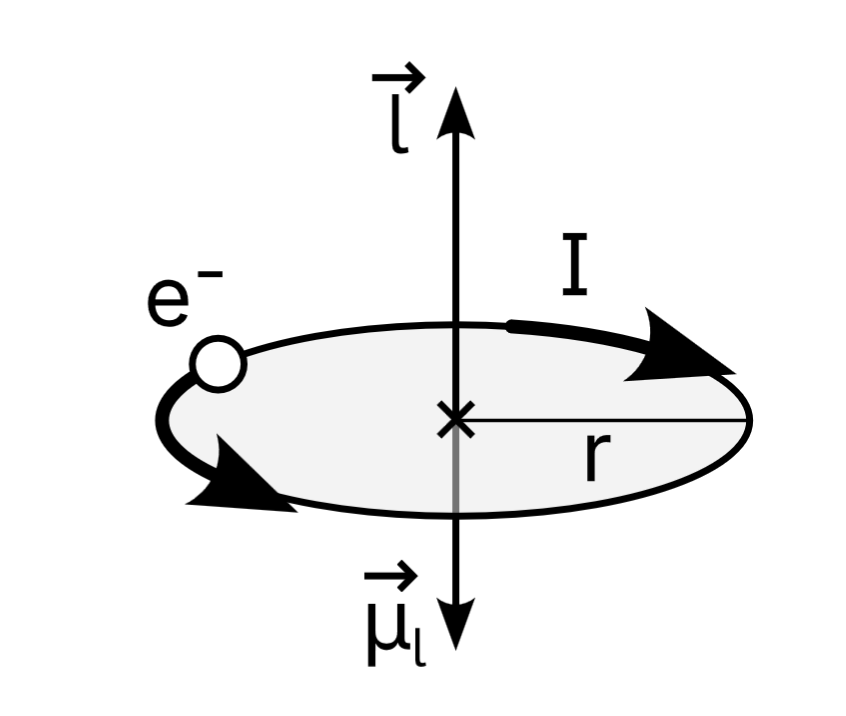
\includegraphics[width=0.25\linewidth]{figures/electron_circular_path.png}
    \caption{An electron moving on a circular orbit generates a current $I$, an orbital angular momentum $\vec{l}$, and a magnetic moment $\vec{\mu}_l$.}
    \label{fig:electron_circular_path}
\end{figure}

The magnetic moment and the orbital angular momentum are related by

\begin{equation}
    \vec{\mu}_l = -\frac{e}{2m_e}\vec{l} = -\gamma_l \vec{l},
    \label{angular_magnetic_moment}
\end{equation}

where $e$ denotes the elementary charge, $m_e$ the electron mass, and

\begin{equation}
    \gamma_l = \frac{e}{2m_e}
\end{equation}

is called the gyromagnetic ratio. The negative sign reflects the fact that the electron carries a negative charge, so the magnetic moment is antiparallel to the angular momentum.

In quantum mechanics, the magnitude of the orbital angular momentum is quantized. It is determined by the azimuthal quantum number $l = 0, 1, 2, \dots, n-1$, where $n = 1, 2, 3, \dots$ is the principal quantum number. The magnitude of the angular momentum vector is then given by

\begin{equation}
    |\vec{l}| = \sqrt{l(l+1)}\hbar.
\end{equation}

The projection of the angular momentum onto the quantization axis, usually chosen as the $z$-axis, is also quantized. It is determined by the magnetic quantum number $m_l = -l, -l+1, \dots, l-1, l$, such that

\begin{equation}
    l_z = m_l \hbar.
\end{equation}

According to the Heisenberg uncertainty principle, it is not possible to simultaneously determine all components of the angular momentum vector with arbitrary precision. Therefore, only one component, usually $l_z$, can be measured exactly at a time.

For visualization, the quantum mechanical angular momentum can be represented as a vector of fixed magnitude whose projection onto the $z$-axis remains constant. In this picture, the vector appears to precess around the quantization axis on a cone-shaped path.

Every electron possesses, in addition to its orbital angular momentum, an intrinsic angular momentum called spin $\vec{s}$, which is quantized by the spin quantum number $s = \frac{1}{2}$:

\begin{equation}
    |\vec{s}| = \sqrt{s(s+1)}\hbar = \frac{\sqrt{3}}{2}\hbar.
\end{equation}

In analogy with the orbital angular momentum $\vec{l}$, the spin gives rise to a magnetic spin moment $\vec{\mu}_s$ given by

\begin{equation}
    \vec{\mu}_s(\vec{s}) = - g_s \frac{e}{2m_e}\vec{s},
\end{equation}

which differs from equation~\eqref{angular_magnetic_moment} by the spin Landé factor $g_s = 2.002319 \approx 2$. This factor arises from relativistic quantum mechanics and leads to the gyromagnetic ratio

\begin{equation}
    \gamma_s = g_s \frac{e}{2m_e} \approx \frac{e}{m_e}.
\end{equation}

In a magnetic field, the spin precesses around the field direction with two possible orientations described by the spin magnetic quantum number $m_s = \pm\frac{1}{2}$, so that $s_z = m_s \cdot \hbar$, as illustrated in figure~\ref{fig:precession_spin_ang_momentum}.


\begin{figure}[h]
    \centering
    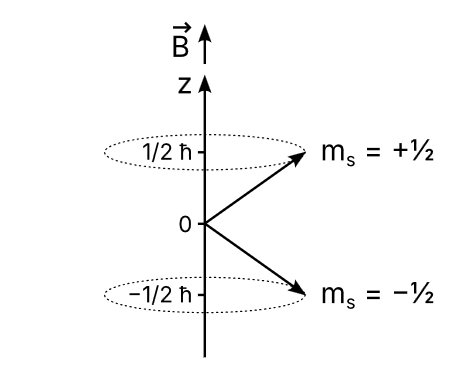
\includegraphics[width=0.5\linewidth]{figures/precession_of_spin_ang_momentum.png}
    \caption{Precession of the spin angular momentum vector $\vec{s}$ in a magnetic field $\vec{B}$}
    \label{fig:precession_spin_ang_momentum}
\end{figure}

When dealing with \textbf{multi-electron systems}, such as heavier atoms, the total orbital angular momentum and the total spin are obtained by vector addition over all electrons:
\begin{equation}
    \vec{L} = \sum_i\vec{l}_i, \qquad \vec{S} = \sum_i \vec{s}_i.
\end{equation}

\paragraph{Atoms in an external magnetic field and spin-orbit coupling}

In atoms with lighter nuclei, the individual orbital angular momenta and spins couple according to the LS (Russell-Saunders) coupling scheme. The total orbital angular momentum $\vec{L}$ and the total spin $\vec{S}$ couple to form the total angular momentum of the atom:
\begin{equation}
    \vec{J} = \vec{L} + \vec{S},
\end{equation}
with magnitude $|\vec{J}| = \sqrt{J(J+1)}\hbar$, where $J = |L-S|, |L-S|+1, \ldots, L+S$ is the total angular momentum quantum number. Because the spin and orbital magnetic moments scale differently with their respective angular momenta (owing to the factor $g_s \approx 2$), the resulting total magnetic moment $\vec{\mu}_J$ is not collinear with $\vec{J}$. Only the component of $\vec{\mu}_J$ along $\vec{J}$ is time-averaged to a non-zero value due to the precession. Its magnitude depends on the quantum numbers $L$, $S$, and $J$ through the general Landé $g$-factor:

\begin{equation}
    g_J = \frac{3J(J+1) + S(S+1) - L(L+1)}{2J(J+1)}.
    \label{eq:lande}
\end{equation}

When an external magnetic field $\vec{B} = (0, 0, B)^T$ is applied, the degeneracy with respect to the magnetic quantum number $M_J = -J, -(J-1), \ldots, J$ is lifted. The potential energy of the magnetic moment in the field is
\begin{equation}
    U = -\vec{\mu}_J \cdot \vec{B} = M_J g_J \mu_B B,
\end{equation}
where the Bohr magneton $\mu_B = \frac{e\hbar}{2m_e} = 9.274 \cdot 10^{-24}$J/T is the natural unit of magnetic moment corresponding to the smallest angular momentum unit $L_z = 1\hbar$. An energy level thus splits into $2J+1$ equidistant sublevels, each separated by
\begin{equation}
    \Delta E = g_J \mu_B B.
\end{equation}
In the external field, the total angular momentum vector $\vec{J}$ precesses around the field direction with the Larmor frequency $\omega_L = g_J\frac{e}{2m_e}B$.

\paragraph{Selection Rules}
Atomic energy states change upon the absorption or emission of a photon. These electric dipole transitions are governed by the following quantum mechanical selection rules:

\begin{itemize}
    \item $\Delta J = 0, \pm 1$ (with the restriction $J = 0 \not\leftrightarrow J = 0$): Because a photon possesses an intrinsic spin of $1\hbar$, the atom must change its total angular momentum to conserve angular momentum during a transition. The case $\Delta J = 0$ is allowed as long as neither level has $J = 0$, since a $J=0 \to J=0$ transition cannot satisfy angular momentum conservation.
    \item $\Delta M_J = 0, \pm 1$: A change in the projection of the angular momentum ($\Delta M_J = \pm 1$) is associated with the emission of circularly polarized light ($\sigma_+$ or $\sigma_-$), whereas a transition preserving the projection ($\Delta M_J = 0$) produces linearly polarized light ($\pi$). Note that the $\Delta M_J = 0$ transition does not violate angular momentum conservation because each photon's spin expectation value is zero, even though each individual photon measurement returns $\pm\hbar$.
    \item $\Delta S = 0$: The total electron spin state generally remains unchanged during an electric dipole transition.
\end{itemize}

Regardless of the actual number of magnetic sublevels, these selection rules ensure that at most three distinct transition energies are observed in the normal Zeeman effect.

\subsubsection{Normal Zeeman Effect}

The normal Zeeman effect occurs for transitions in which the total spin of both levels involved is zero, i.e.\ $S = 0$. As a consequence, $J = L$ and the Landé $g$-factor from equation~\eqref{eq:lande} reduces to $g_J = g_L = 1$ for both levels. The energy of each sublevel is then
\begin{equation}
    E = E_{n,L} + M_L\mu_BB,
\end{equation}
and the sublevel spacing $\Delta E = \mu_B B$ is identical for both involved levels. The selection rule $\Delta M_L = 0, \pm 1$ then gives rise to exactly three spectral lines regardless of the quantum numbers of the levels.

\paragraph{Classical picture}
Hendrik Lorentz explained the normal Zeeman effect using a purely classical oscillator model.
\begin{figure}[h]
    \centering
    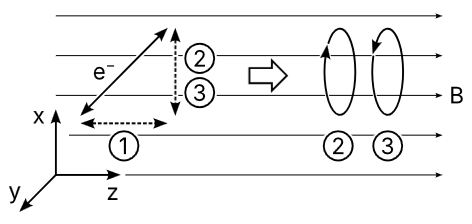
\includegraphics[width=0.75\linewidth]{nomrla_zeemann_classical_approch.png}
    \caption{An Electron as oscilator in a magnetic field $\vec{B}$ (classical approch)}
    \label{fig:nomrla_zeemann_classical_approch}
\end{figure}
A light-emitting electron is treated as a harmonic oscillator of resonance frequency $\omega_0$. In the presence of a magnetic field $\vec{B} = (0, 0, B)^T$, the equation of motion is
\begin{equation}
    m_e\ddot{\vec{r}} = -k\vec{r} + e\dot{\vec{r}} \cdot \vec{B},
\end{equation}
where the second term accounts for the Lorentz force. Decomposing the motion into components parallel and perpendicular to $\vec{B}$, the $z$-component (parallel) is unaffected by the magnetic field and oscillates at the original frequency $\omega_0$. Introducing the complex coordinate $u = x + iy$ to decouple the perpendicular equations and applying the approximation $\omega_L \ll \omega_0$, where $\omega_L = eB/2m_e$ is the Larmor frequency, two circularly polarized modes are found:
\begin{equation}
    \omega_+ = \omega_0 + \omega_L \qquad \text{and} \qquad \omega_- = \omega_0 - \omega_L.
\end{equation}
This leads to three oscillation modes, a linear oscillator at $\omega_0$ that is parallel to $\vec{B}$ and two counter-rotating circular oscillators at $\omega_\pm$ in the plane perpendicular to $\vec{B}$.

\paragraph{Observation directions}
\begin{figure}[h]
    \centering
    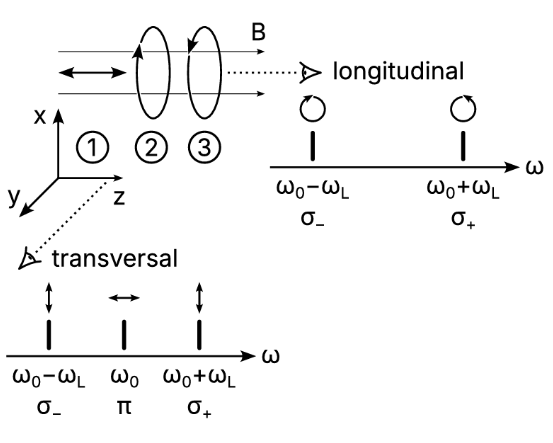
\includegraphics[width=0.75\linewidth]{direction_normal.png}
    \caption{Transversal a longitudinal direction for the normal Zeeman effect}
    \label{fig:direction_normal}
\end{figure}
Depending on the direction of observation, different polarizations are detected. In the transversal direction which is perpendicular to $\vec{B}$, all three modes are visible as linearly polarized light. The central $\pi$ line, from the $z$-oscillator, polarized parallel to $\vec{B}$, and the two $\sigma_\pm$ lines at $\omega_\pm$ that are appearing as linear projections of the circular motion. In the longitudinal direction that is parallel to $\vec{B}$, the $\pi$ oscillator radiates no light along its axis, so only two lines remain, observed as left- and right-circularly polarized $\sigma_+$ and $\sigma_-$ radiation.

\begin{figure}[h]
    \centering
    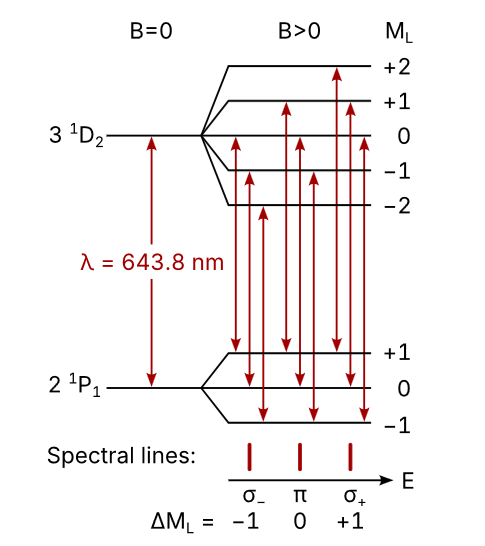
\includegraphics[width=0.75\linewidth]{figures/transition_normal.png}
    \caption{Energy level diagram for the transition $3^1D_2 \leftrightarrow 2^1P_1$ in the cadmium atom}
    \label{fig:transition_normal}
\end{figure}

In this experiment, the transition $3^1D_2 \leftrightarrow 2^1P_1$ of cadmium at $\lambda = 643.8$nm is used to observe the normal Zeeman effect. For $3^1D_2$ ($J = 2$, $S = 0$) and $2^1P_1$ ($J = 1$, $S = 0$), one has $g_J = 1$ for both levels, giving exactly three spectral components with $\Delta E = \mu_B B$. As shown in figure~\ref{fig:transition_normal}.

\subsubsection{Anomalous Zeeman Effect}

For transitions involving levels with non-zero total spin $S > 0$, the Landé $g$-factor is no longer equal to 1 as in the normal Zeeman effect. As a result, the spacing between adjacent sublevels differs on the two sides of the transition, and more than three spectral lines can appear. This is the anomalous Zeeman effect. The energy of each sublevel is
\begin{equation}
    E = E_{n,L} + M_J g_J \mu_B B,
\end{equation}
and the $2J+1$ sub-level values of $M_J$ for each level lead to up to $2J+1$ distinct energies. The selection rule $\Delta M_J = 0, \pm 1$ then permits transitions between these sub-levels.

\begin{figure}[h]
    \centering
    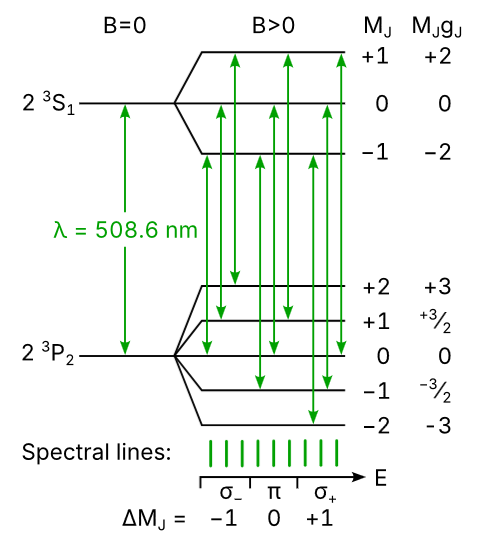
\includegraphics[width=0.75\linewidth]{figures/transition_azeemann.png}
    \caption{Energy level diagram for the transition $2^3S_1 \leftrightarrow 2^3P_2$ in the cadmium atom}
    \label{fig:transition_annoumalus}
\end{figure}



This experiment shows the cadmium transition $2^3S_1 \leftrightarrow 2^3P_2$ at $\lambda = 508.6$ nm. The $2^3S_1$ energy level splits into three sublevels ($M_J \in \{-1, 0, +1\}$) with a Landé g-factor of $g_J = 2$, while the $2^3P_2$ level splits into five sublevels ($M_J \in \{-2, -1, 0, +1, +2\}$) with $g_J = 3/2$. Following the selection rule $\Delta M_J = 0, \pm 1$, these levels split into nine distinct transition lines, each equally spaced by $\frac{1}{2}\mu_B B$. When viewing the system transversely, all nine lines can theoretically be seen, but when viewing it longitudinally, the three $\pi$ transitions ($\Delta M_J = 0$) disappear, leaving only the six $\sigma_\pm$ lines visible.

\subsubsection{Optical Polarizers}

\paragraph{Linear polarization filter} A linear polarizer transmits only the component of the electric field oscillating along a single, fixed direction, blocking all orthogonal components. If linearly polarized light of intensity $I_0$ is incident on a linear polarizer, the transmitted intensity follows Malus' law:
\begin{equation}
    I = I_0\cos^2(\alpha),
\end{equation}
where $\alpha$ is the angle between the polarization direction of the incident light and the transmission axis of the filter. If the incident light is unpolarized or circularly polarized, the transmitted intensity is independent of $\alpha$.

\paragraph{Quarter-wave plate} A quarter-wave plate (QWP) is made from a birefringent crystal with two orthogonal optical axes, the fast axis (lower refractive index $n_1$) and the slow axis (higher refractive index $n_2$). Light passing through the plate accumulates a relative phase shift between the components polarized along these two axes of
\begin{equation}
    \Delta\varphi = \frac{2\pi d}{\lambda_0}|n_1 - n_2|,
\end{equation}
where $d$ is the plate thickness and $\lambda_0$ the vacuum wavelength. The thickness of a quarter-wave plate is chosen such that $\Delta\varphi = \pi/2$ in other words a quarter of a full oscillation. When linearly polarized light enters the quarter-wave plate with its polarization plane at $45°$ to the fast axis, the two components emerge with equal amplitude but a phase difference of $\pi/2$, producing circularly polarized light. Conversely, when circularly polarized light passes through a QWP, it is converted into linearly polarized light. This conversion property is exploited in this experiment to distinguish left- and right-circularly polarized $\sigma_+$ and $\sigma_-$ components.

\subsubsection{Resolving Power}

The resolving power $\lambda/\Delta\lambda$ quantifies the smallest wavelength difference $\Delta\lambda$ that can still be distinguished from a reference wavelength $\lambda$ by an optical instrument. Two spectral lines at wavelengths $\lambda$ and $\lambda + \Delta\lambda$ are considered just resolvable when $\Delta\lambda$ equals the minimum distinguishable separation.

The energy difference corresponding to a wavelength separation $\Delta\lambda$ is obtained via
\begin{equation}
    \Delta E = \frac{hc}{\lambda^2}\Delta\lambda \quad \Rightarrow \quad \frac{\lambda}{\Delta\lambda} = \frac{hc}{\Delta E\lambda}.
    \label{eq:resolving_general}
\end{equation}

In the longitudinal configuration (where only $\sigma_\pm$ lines are visible and the $\pi$ line is absent), adjacent rings correspond to a total energy separation $\Delta E = 2\mu_B B$. The experimental resolving power is therefore
\begin{equation}
    \frac{\lambda}{\Delta\lambda} = \frac{hc}{2\mu_B B\lambda},
    \label{eq:resolving_exp}
\end{equation}
where $B$ is the magnetic flux density at which two neighboring rings can just be resolved.

For the Fabry-Pérot interferometer, the theoretical resolving power is set by the width of the transmission peaks. A detailed derivation (see Section~\ref{sec:fabrypérot}) yields
\begin{equation}
    \left(\frac{\lambda}{\Delta\lambda}\right)_\mathrm{theo} = \frac{2\pi d\sqrt{R}}{\lambda(1-R)},
    \label{eq:resolving_theo}
\end{equation}
where $d$ is the mirror spacing, $R$ the mirror reflectivity, and $\lambda$ the wavelength.

\subsubsection{Fabry-Pérot Interferometer}
\label{sec:fabrypérot}

\begin{figure}
    \centering
    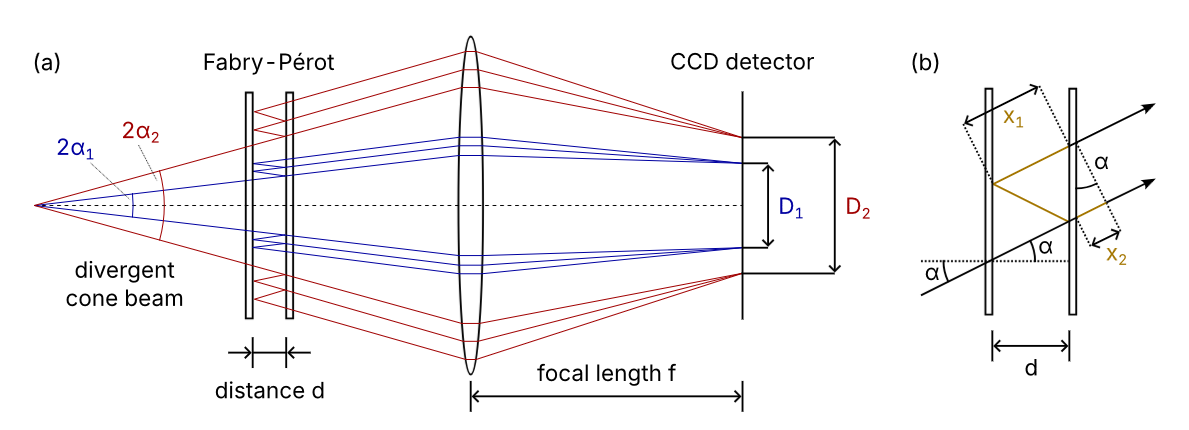
\includegraphics[width=0.75\linewidth]{figures/interferrometer.png}
    \caption{(a) figure shows the Fabry-Pérot interferometer, and it's passing beam path, (b) The geometry for constructing the path difference}
    \label{fig:interferrometer}
\end{figure}

The Fabry-Pérot interferometer consists of two flat, parallel glass plates separated by a distance $d$, whose inner surfaces are coated with semi-transparent mirrors of reflectivity $R$. Light enters as a divergent cone beam and undergoes multiple reflections between the plates. The superposition of all transmitted partial waves gives constructive interference when the optical path difference between successive reflections is an integer multiple of the wavelength:
\begin{equation}
    m\lambda = 2d\cos\alpha,
    \label{eq:interference_condition}
\end{equation}
where $m$ is the (integer) interference order and $\alpha$ is the angle of incidence. Since different wavelengths satisfy this condition at different angles $\alpha$, the interference image of a polychromatic source consists of concentric rings of different radii. For small angles, the ring diameter $D$ is related to $\alpha$ by $D \approx 2f\alpha$, where $f$ is the focal length of the imaging lens.

The transmission function of the Fabry-Pérot interferometer as a function of the light frequency $f$ takes the form
\begin{equation}
    \mathbb{T}(f) = \frac{1}{1 + \dfrac{4R}{(1-R)^2}\sin^2\!\left(\dfrac{2\pi d}{c}f\right)},
\end{equation}
which shows sharp transmission maxima separated by the free spectral range $\mathrm{FSR} = c/2d$. Close to a resonance, the transmission peak has a full width at half maximum (FWHM) of $\mathrm{FSR}/\mathcal{F}$, where the finesse $\mathcal{F} = \pi\sqrt{R}/(1-R)$ is a dimensionless figure of merit that increases with mirror reflectivity. The theoretical resolving power is then obtained by requiring two frequencies to be separated by at least one FWHM, leading to equation~\eqref{eq:resolving_theo}.

The energy splitting between two spectral lines (corresponding to two rings of diameters $D_1$ and $D_2$ within the same interference order $m$, and rings of diameters $D_{1,m+1}$ and $D_{2,m+1}$ in the adjacent order $m+1$) is given by
\begin{equation}
    \Delta E = \frac{hc}{2d}\left[\frac{D_{1,m}^2}{D_{1,m+1}^2 - D_{1,m}^2} - \frac{D_{2,m}^2}{D_{2,m+1}^2 - D_{2,m}^2}\right].
    \label{eq:delta_E_transversal}
\end{equation}
In the longitudinal configuration, only the outer ($\sigma_+$) and inner ($\sigma_-$) rings are visible, with the $\pi$ ring absent. Because these two rings correspond to a total energy separation of $\Delta E_\mathrm{obs} = 2\mu_B B$, the formula must be divided by an additional factor of 2 to recover the energy splitting between adjacent sub-levels:
\begin{equation}
    \Delta E = \frac{hc}{4d}\left[\frac{D_{1,m}^2}{D_{1,m+1}^2 - D_{1,m}^2} - \frac{D_{3,m}^2}{D_{3,m+1}^2 - D_{3,m}^2}\right],
    \label{eq:delta_E_longitudinal}
\end{equation}
where $D_{1,m}$ and $D_{3,m}$ denote the diameters of the outer and inner ring in interference order $m$, respectively.

\subsubsection{Hall Sensor}

At the beginning of the experiment, the magnetic flux density between the pole pieces is calibrated as a function of the coil current using a Hall effect sensor.
With a rough schematic in figure~\ref{fig:hall_sensor} the sensor consists of an n-doped GaAs crystal through which a known current $I_H$ flows. In a perpendicular magnetic field $B$, the Lorentz force on the charge carriers creates a transverse charge separation, which in turn produces a measurable Hall voltage $U_H = A_H \frac{I_H}{d} B$, where $A_H$ is the material-specific Hall constant and $d$ the sensor thickness. The Hall voltage is thus proportional to $B$, enabling a precise measurement of the magnetic flux density.

\begin{figure}
    \centering
    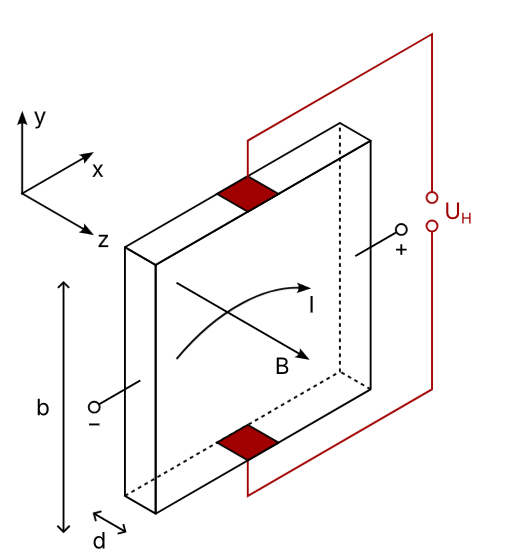
\includegraphics[width=0.75\linewidth]{figures/hall_sensor.png}
    \caption{Basic schematic of the setup of a Hall effect sensor}
    \label{fig:hall_sensor}
\end{figure}

\subsection{Experimental Setup}
\begin{figure}[h]
    \centering
    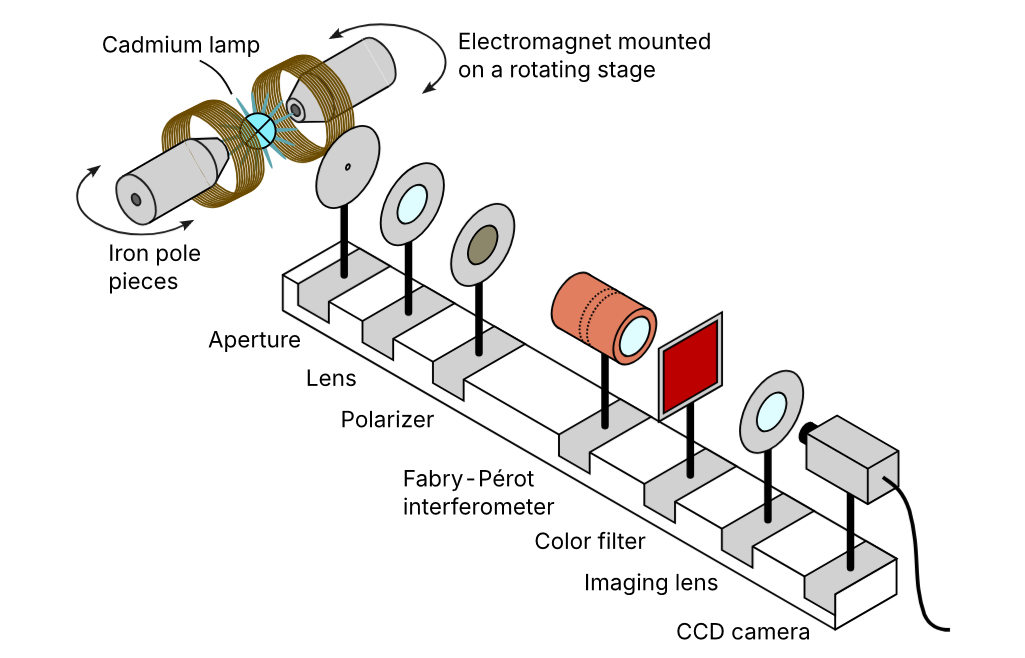
\includegraphics[width=0.75\linewidth]{figures/experimental_setup.png}
    \caption{Schematic of the experimental setup. From left to right: cadmium spectral lamp in the iron pole pieces of the electromagnet (mounted on a rotating stage), aperture, collimating lens, optional polarization filter assembly, Fabry-Pérot interferometer, color filter, imaging lens, and CCD camera.}
    \label{fig:setup}
\end{figure}

The experimental setup is shown in figure~\ref{fig:setup}. The cadmium spectral lamp is positioned between the iron pole pieces of an electromagnet. The pole pieces are magnetized by the coil field and thereby amplify the flux density in the region of the lamp. The entire magnet and lamp assembly is mounted on a rotating stage, allowing the direction of observation to be switched between transversal, that is perpendicular to $\vec{B}$, and longitudinal, that is parallel to $\vec{B}$. In the longitudinal orientation, the light exits through small holes in the pole pieces.

The emitted light first passes through an aperture, which approximates a point light source. A collimating lens then directs as much light as possible into the Fabry-Pérot interferometer as a quasi-parallel beam. The interferometer itself contains an entrance lens that generates the divergent cone beam required to produce ring-shaped interference patterns. After the interferometer, a color filter selects the desired transition. A red absorption filter for $\lambda = 643.8$nm the normal Zeeman effect and a narrowband interference filter for $\lambda = 508.6$nm the anomalous Zeeman effect. An imaging lens finally focuses the interference image onto the CCD sensor of the camera, and the resulting image is displayed on a computer for analysis with ImageJ.

\section{Results and Discussion}

\subsection{Calibrating the magnetic fields}
\subsubsection{Magnetic flux density over the current}

\begin{figure}[h]
    \centering
    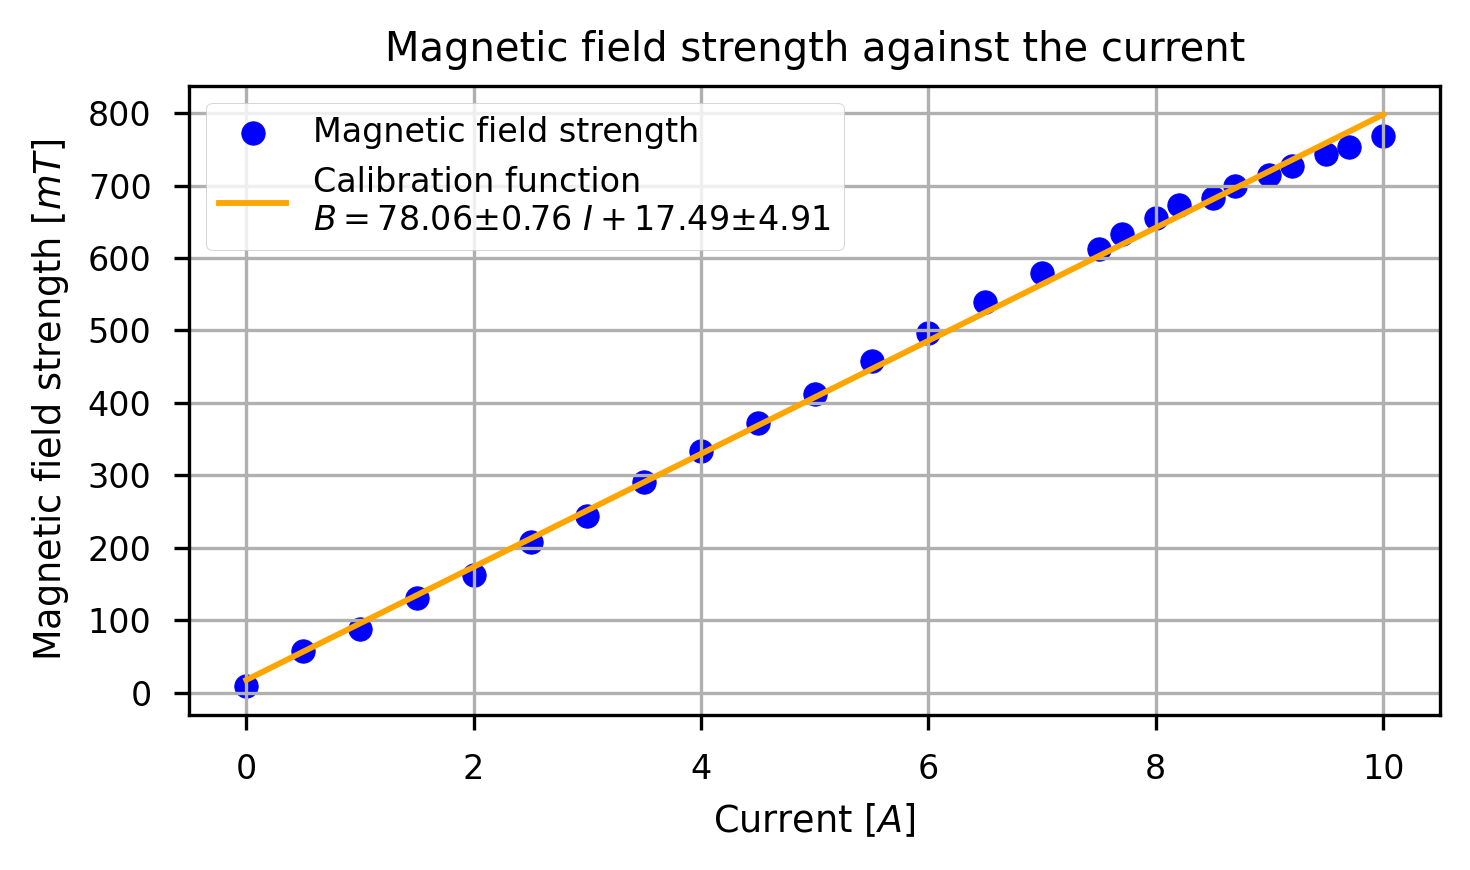
\includegraphics[width=0.8\linewidth]{figures/magnetic_field_strength_against_the_current.png}
    \caption{Magnetic flux density $B$ as a function of the coil current $I$. A linear fit is shown as a dashed line. A slight deviation from linearity is visible at currents above approximately 8A, indicating the onset of magnetic saturation of the iron pole pieces.}
    \label{fig:magnetic_filed_strength_against_current}
\end{figure}

The magnetic flux density was measured in the center between the two pole pieces as a function of the coil current from 0A to 10A, and the result is shown in figure~\ref{fig:magnetic_filed_strength_against_current}. The relationship is approximately linear over most of the measurement range, as expected from Ampère's law for a coil with iron core in the unsaturated regime ($B \propto I$). The linear calibration function obtained from a least-squares fit is

\begin{equation}
    B(I) = 78.06\frac{\mathrm{mT}}{\mathrm{A}} \cdot I + 17.49\mathrm{mT}.
    \label{current_to_flux_formula}
\end{equation}

A small but visible deviation from linearity emerges at currents above approximately 8A, where the iron pole pieces begin to approach magnetic saturation. At this point, nearly all microscopic magnetic domains within the iron are aligned with the applied field, so further increases in coil current produce progressively smaller increments in $B$. As shown in the calibration table below, the maximum deviation between the linear fit and the measured values remains below 9\% over the entire range. Because this deviation is relatively small, equation~\eqref{current_to_flux_formula} is used throughout this report as the conversion formula. A polynomial fit of higher degree would reduce the residuals further but is not necessary for the level of precision required here.

\begin{table}[!ht]
    \centering
    \begin{tabular}{rrll}
    \hline
        \textbf{I [A]} & \textbf{B [mT]} & \textbf{Fit [mT]} & \textbf{Deviation [\%]} \\ \hline \hline
        0 & 9 & 17.49 & 94.33 \\ \hline
        1 & 88 & 95.55 & 8.58 \\ \hline
        2 & 163 & 173.61 & 6.51 \\ \hline
        3 & 244 & 251.67 & 3.14 \\ \hline
        4 & 334 & 329.73 & 1.28 \\ \hline
        5 & 413 & 407.79 & 1.26 \\ \hline
        6 & 497 & 485.85 & 2.24 \\ \hline
        7 & 579 & 563.91 & 2.61 \\ \hline
        8 & 655 & 641.97 & 1.99 \\ \hline
        9 & 715 & 720.03 & 0.70 \\ \hline
        10 & 769 & 798.09 & 3.78 \\ \hline
    \end{tabular}
    \caption{Measured magnetic flux densities, values computed from the linear calibration fit, and the relative deviation between measurement and fit for each coil current.}
\end{table}

\subsubsection{Spatial profile of the magnetic flux density}

In this section, the spatial profile of the magnetic flux density perpendicular to the magnetic field direction was investigated. For this purpose, the magnetic flux density $B$ was measured as a function of the position $x$ using a Hall sensor at a constant current of $I = 10$A. The zero point of the position scale was chosen to lie at the center between the two pole pieces.

The measured data were fitted using a polynomial. The resulting spatial magnetic field profiles are shown in figure~\ref{fig:spatial_profile}, both as a summary for currents from 1A to 10A (figure~\ref{fig:spatial_profile_summary}) and in detail for $I = 10$A (figure~\ref{fig:spatial_profile_10A}).

\begin{figure}[h]
    \begin{subfigure}{0.49\textwidth}
    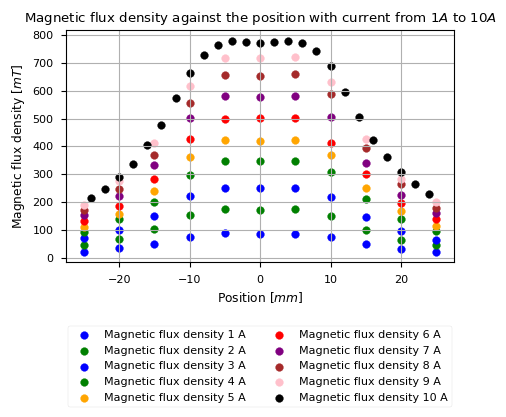
\includegraphics[width=1\linewidth]{figures/spatial_profile_against_postion_summary.png}
    \caption{Spatial profiles of the magnetic flux density for currents from $1$A to $10$A}
    \label{fig:spatial_profile_summary}
    \end{subfigure}
    \begin{subfigure}{0.5\textwidth}
    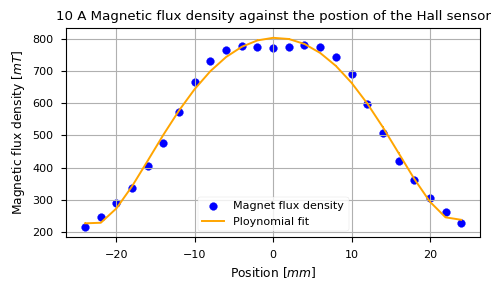
\includegraphics[width=1\linewidth]{figures/spatial_profile_magentic_flux_density_10A.png}
    \caption{Spatial profile of the magnetic flux density at $I = 10$A}
    \label{fig:spatial_profile_10A}
    \end{subfigure}
\caption{Spatial profiles of the magnetic flux density measured with the Hall sensor as a function of position $x$.}
\label{fig:spatial_profile}
\end{figure}

In all measurement series ($1$A to $10$A), a distinct, localized "dip" in the magnetic flux density is observed directly at the center ($x = 0$ mm), caused by the specific geometry of the pole pieces and the spatial redistribution of the flux lines, is a physical phenomenon often seen in electromagnet setups with parallel pole pieces. While the magnetic field is highly concentrated between the poles, the magnetic flux lines tend to "dip" slightly at the very center of the gap to minimize total magnetic reluctance. Furthermore, the pole pieces had slight geometric features as a central borehole where the field can exhibit a local minimum. The 6th-grade polynomial fit fails to adapt to this central minimum because it prioritizes mapping the steep drop-offs at the outer edges. Even testing higher-degree polynomial fits did not resolve this issue. However, because the total spatial deviation near the cadmium lamp remains well below $10\%$, this central dip can be ignored, and the magnetic field can still be considered sufficiently homogeneous for the purposes of this experiment.

\subsection{Normal Zeeman Effect}

Interference images were recorded with the CCD camera for the normal Zeeman effect at $\lambda = 643.8$nm using a red absorption filter. The coil current was increased in steps of 1A from 1A to 10A, and the corresponding magnetic flux densities were determined using the calibration function~\eqref{current_to_flux_formula}. Both the transversal and longitudinal observation configurations were investigated, first without any polarization filter and then with a linear polarizer and, additionally, a quarter-wave plate.

\subsubsection{Transversal configuration}

In the transversal configuration, the rotating magnet is oriented perpendicular to the optical axis so that $\vec{B}$ is perpendicular to the direction of observation. figure~\ref{fig:normal_zeeman_transversal} shows a pie chart of the interference patterns recorded at different coil currents (converted to magnetic flux densities using equation~\eqref{current_to_flux_formula}).

\begin{figure}[h]
    \centering
    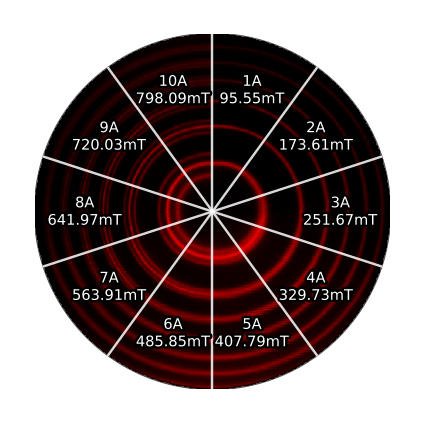
\includegraphics[width=0.6\linewidth]{figures/normal_zeeman_transversal.png}
    \caption{Pie chart of the interference patterns of the normal Zeeman effect in the transversal direction, without a polarization filter, for various coil currents and the corresponding magnetic flux densities.}
    \label{fig:normal_zeeman_transversal}
\end{figure}

The interference rings were analyzed with the scientific image-processing software ImageJ. The pie chart was assembled from individual images using a custom Python script. The normalized radial intensity profiles for the lowest ($1\mathrm{A} \approx 95.55$mT) and highest ($10\mathrm{A} \approx 798.09$mT) currents are shown in figure~\ref{fig:transversal_norm_plot}.

\begin{figure}[h]
    \centering
    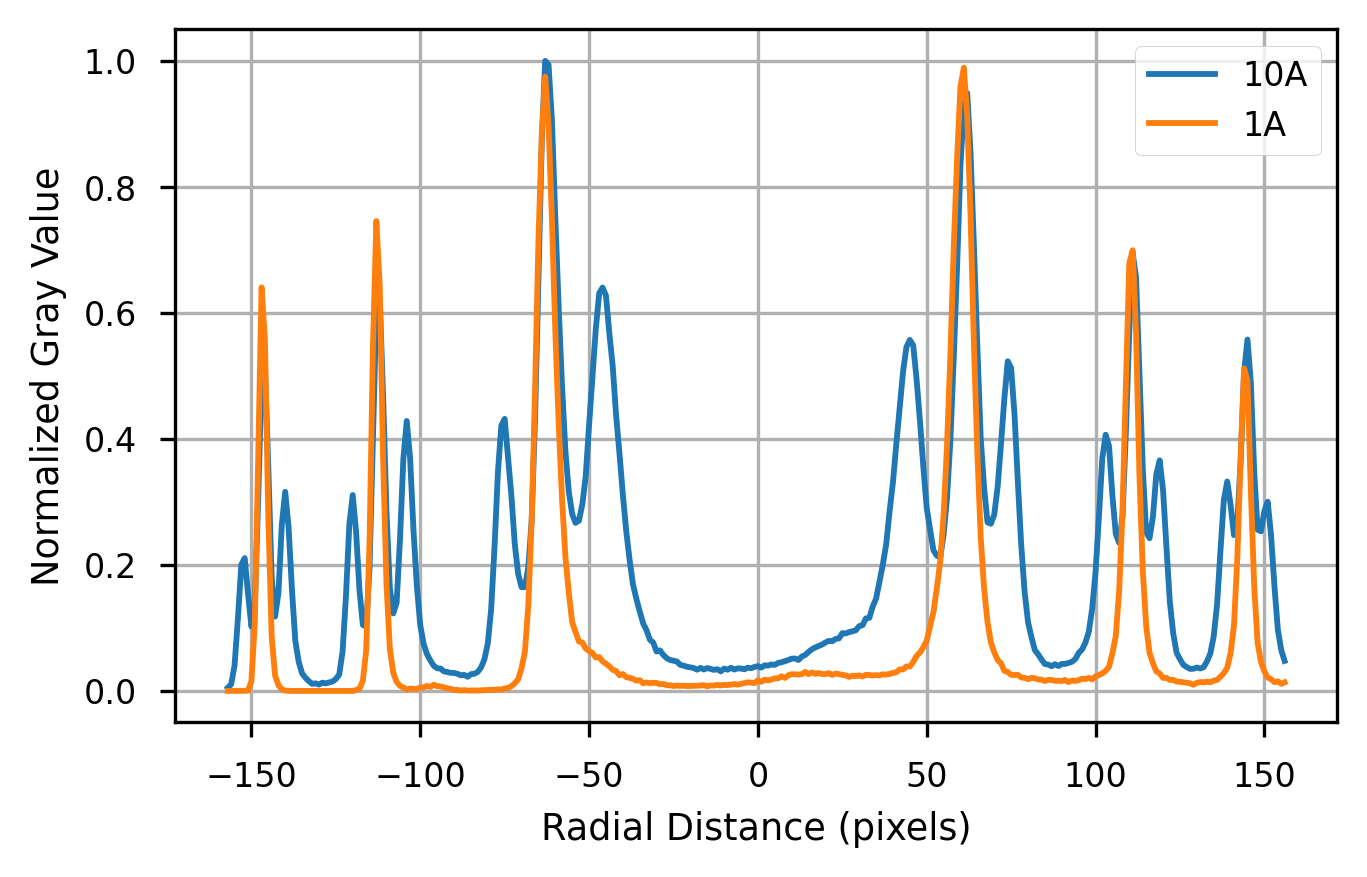
\includegraphics[width=0.8\linewidth]{figures/normalized_intensity_transversal_normal.png}
    \caption{Normalized intensity $I/I_\mathrm{max}$ as a function of radial distance from the ring center for the normal Zeeman effect in the transversal direction (without polarization filter) at $1\mathrm{A} \approx 95.55$mT and $10\mathrm{A} \approx 798.09$mT.}
    \label{fig:transversal_norm_plot}
\end{figure}

At very low magnetic flux densities, only a single interference maximum per order is visible for each wavelength, as the Zeeman splitting is smaller than the instrumental resolution. As the flux density increases, each original ring splits into three distinct sub-rings. The central $\pi$ ring remains at a constant radial position independent of $B$, while the inner and outer rings ($\sigma_-, \, \sigma_+$) move symmetrically away from the center in proportion to $B$. This behavior is fully consistent with the theoretical prediction for the normal Zeeman effect as the energy levels split equidistantly by $\Delta E = \mu_B B$, so that the three allowed transitions ($\Delta M_L = 0, \pm 1$) show three spectral lines displaced by equal amounts on either side of the original line. In the transversal direction, all three components are visible as linearly polarized light.

The overall brightness of the rings also increases slightly with current. This is likely because the stronger magnetic field confines the ion trajectories in the gas discharge into tighter helical paths, increasing the collision frequency between ions and neutral atoms and thereby enhancing the excitation and emission rate.

To identify the polarization of the individual rings, a linear polarizer and subsequently a quarter-wave plate were introduced into the beam path between the collimating lens and the Fabry-Pérot interferometer. The fast axis of the quarter-wave plate was fixed at $\phi = 45°$ to the vertical, and the transmission axis of the linear polarizer was set to $\theta = 0°$, $45°$, and $90°$, respectively. The resulting images are shown in figure~\ref{fig:transversal_normal_lambda4}.

\begin{figure}[h]
    \begin{subfigure}{0.49\textwidth}
    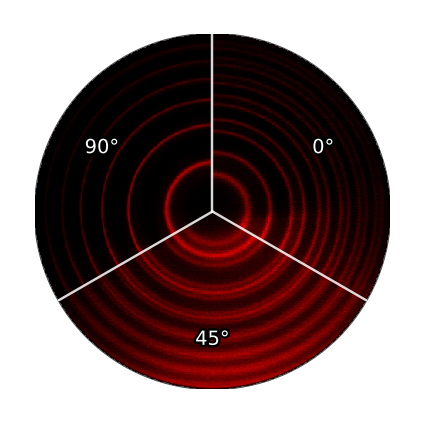
\includegraphics[width=0.75\linewidth]{figures//normal_zeeman_effect/zeemann_transversal_polarisation.png}
    \caption{With a linear polarizer only}
    \label{fig:transversal_normal_polarization}
    \end{subfigure}
    \begin{subfigure}{0.5\textwidth}
    
\includegraphics[width=0.75\linewidth]{figures//normal_zeeman_effect/zeemann_transversal_lambda4_polarisation.png}
    \caption{With a linear polarizer and a quarter-wave plate at $\phi = 45°$}
    \label{fig:transversal_normal_lambda4_sub}
    \end{subfigure}
\caption{Interference patterns of the normal Zeeman effect in the transversal configuration at $798.09$mT with polarization filter angles $\theta = [0°, 45°, 90°]$.}
\label{fig:transversal_normal_lambda4}
\end{figure}

With the linear polarizer alone, the intensities of the outer and inner $\sigma_\pm$ rings extinguish completely at $\theta = 90°$, while the central $\pi$ ring extinguishes at $\theta = 0°$. The polarization directions of the $\sigma_\pm$ rings and the $\pi$ ring are therefore perpendicular to each other ($\Delta\theta = 90°$), confirming that the $\pi$ radiation is polarized parallel to $\vec{B}$ and the $\sigma_\pm$ radiation is polarized perpendicular to $\vec{B}$. At the intermediate angle $\theta = 45°$, both rings show reduced intensity consistent with Malus' law. This observation is in full agreement with the classical and quantum mechanical descriptions of the normal Zeeman effect in the transversal configuration.

When the quarter-wave plate is additionally inserted, the intensity of each ring becomes independent of the polarizer angle $\theta$. This is expected in the transversal direction, the $\pi$ and $\sigma_\pm$ components are all linearly polarized; after passing through the QWP at $\phi = 45°$, each linearly polarized component is converted into elliptically (or circularly) polarized light, so rotation of the subsequent linear polarizer no longer modulates the intensity.

\subsubsection{Longitudinal configuration}

In the longitudinal configuration, the magnet is rotated so that $\vec{B}$ is parallel to the optical axis. Light exits through the bores in the pole pieces. figure~\ref{fig:normal_zeeman_longitudinal} shows the corresponding pie chart, and figure~\ref{fig:normalized_intensity_transversal} shows the radial intensity profiles.

\begin{figure}[h]
    \centering
    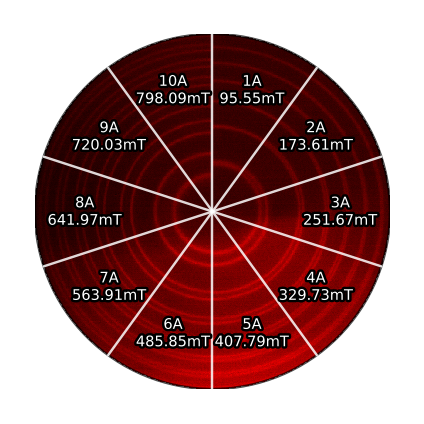
\includegraphics[width=0.75\linewidth]{figures//normal_zeeman_effect/zeeman_longitudinal.png}
    \caption{Pie chart of the interference patterns of the normal Zeeman effect in the longitudinal direction, without a polarization filter, for various coil currents and the corresponding magnetic flux densities.}
    \label{fig:normal_zeeman_longitudinal}
\end{figure}

\begin{figure}[h]
    \centering
    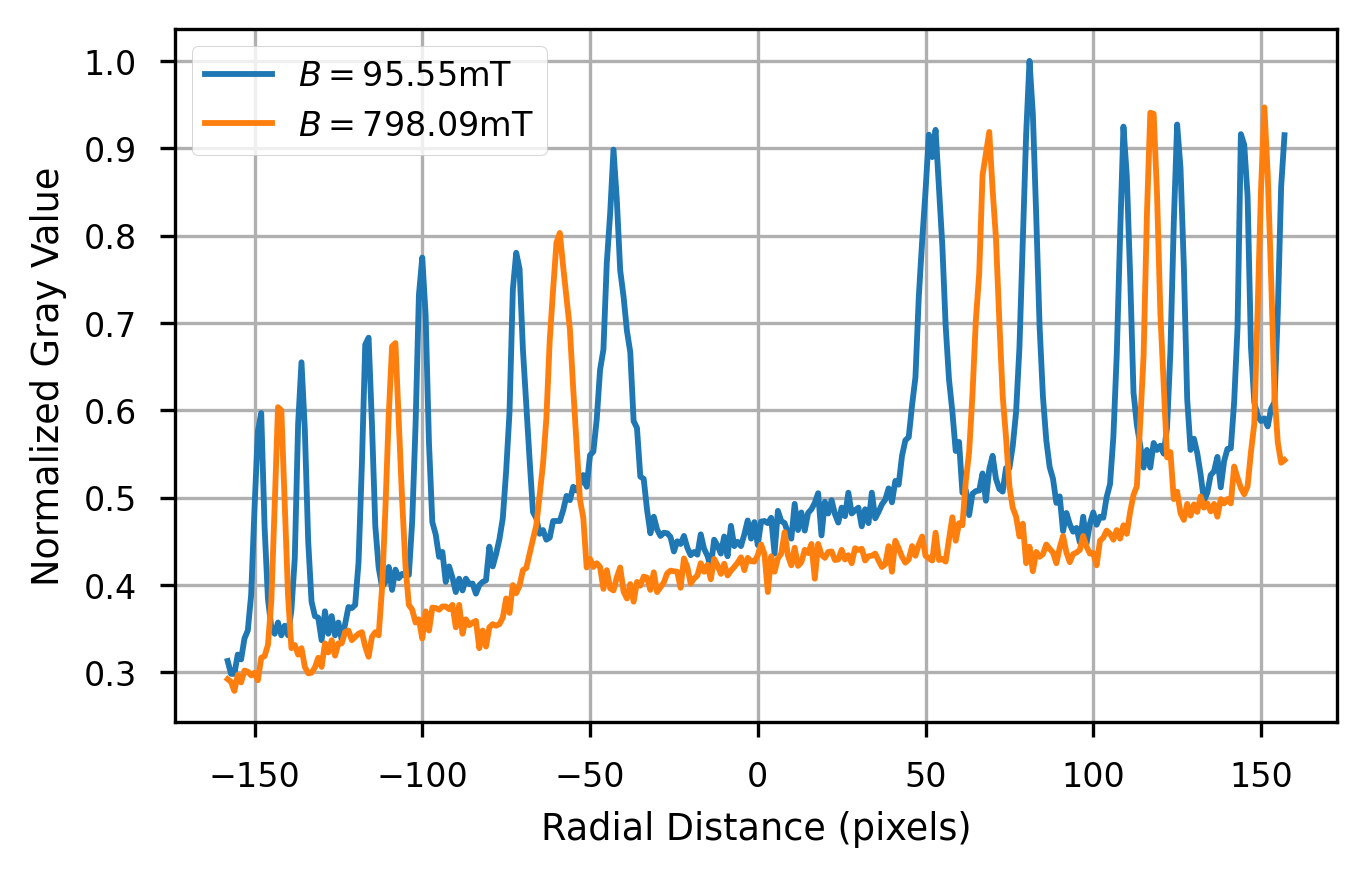
\includegraphics[width=0.75\linewidth]{figures//normal_zeeman_effect/normalized_intensity_transversal.png}
    \caption{Normalized intensity $I/I_\mathrm{max}$ as a function of radial distance from the ring center for the normal Zeeman effect in the longitudinal direction (without polarization filter) at $1\mathrm{A} \approx 95.55$mT and $10\mathrm{A} \approx 798.09$mT. The slight increase in background intensity towards large radii is attributed to stray light from the slightly contaminated optical elements.}
    \label{fig:normalized_intensity_transversal}
\end{figure}

As expected from theory, the longitudinal direction shows a qualitatively different splitting pattern compared to the transversal case. In the longitudinal direction, the $\pi$ component ($\Delta M_L = 0$) does not radiate along the magnetic field axis because the corresponding classical oscillator vibrates parallel to $\vec{B}$ and therefore has no transverse radiation component. Consequently, each single ring observed at zero field splits into only \textit{two} sub-rings as the current is increased, and no central ring is present. The two visible $\sigma_\pm$ rings separate symmetrically from the original position, with the gap between them growing proportionally to $B$.

Because the $\pi$ ring is absent, the energy separation between the observed inner and outer rings is $\Delta E_\mathrm{obs} = 2\mu_B B$ (twice the single-sublevel spacing). This must be taken into account when computing the actual Zeeman splitting from the ring diameters using equation~\eqref{eq:delta_E_longitudinal}, which already incorporates the factor of $1/4d$ rather than $1/2d$.

The slight linear increase in the background intensity visible on one side of figure~\ref{fig:normalized_intensity_transversal} is due to residual contamination on the optical surfaces, like dust on lenses or the color filter, which could led to a slight asymmetry in the scattered light.

Figure~\ref{fig:transversal_normal_lambda4} shows the interference images recorded with the linear polarizer and with the linear polarizer plus the quarter-wave plate at $B = 798.09$mT.

\begin{figure}[h]
    \begin{subfigure}{0.49\textwidth}
    
\includegraphics[width=0.75\linewidth]{figures//normal_zeeman_effect/zeemann_longitudinal_polarisation.png}
    \caption{With a linear polarizer only}
    \label{fig:long_pol_linear}
    \end{subfigure}
    \begin{subfigure}{0.5\textwidth}
    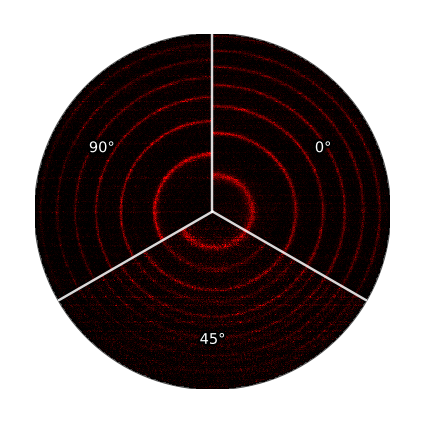
\includegraphics[width=0.75\linewidth]{figures//normal_zeeman_effect/zeemann_longitudinal_lambda4_polarisation.png}
    \caption{With a linear polarizer and a quarter-wave plate at $\phi = 45°$}
    \label{fig:long_pol_lambda4}
    \end{subfigure}
\caption{Interference patterns of the normal Zeeman effect in the longitudinal configuration at $798.09$mT with polarization filter angles $\theta = [0°, 45°, 90°]$.}
\label{fig:transversal_normal_lambda4_long}
\end{figure}

Without the quarter-wave plate, the two rings show equal intensity regardless of the polarizer angle $\theta$. This is consistent with the emission being circularly polarized. A linear polarizer transmits half the intensity of circularly polarized light irrespective of its orientation angle. With the quarter-wave plate inserted, the QWP converts the left- and right-circularly polarized $\sigma_+$ and $\sigma_-$ components into two orthogonally linearly polarized beams. The subsequent linear polarizer then alternately extinguishes the inner and outer ring as $\theta$ is rotated, with the two rings exhibiting intensity maxima exactly $90°$ apart ($\Delta\theta = 90°$). This directly confirms that the $\sigma_+$ and $\sigma_-$ components are circularly polarized with opposite helicity, in full agreement with the quantum mechanical picture.

\subsection{Anomalous Zeeman Effect}

Interference images were recorded at $\lambda = 508.6$nm using a narrowband green interference filter to select the transition $2^3S_1 \leftrightarrow 2^3P_2$. Based on the theoretical analysis in Section~1.2.2, a splitting into nine spectral lines is expected in the transversal direction and into six lines in the longitudinal direction.

\begin{figure}[h]
    \centering
    
\includegraphics[width=0.75\linewidth]{figures//normal_zeeman_effect/zeemann_annormal_transversal.png}
    \caption{Pie chart of the interference patterns of the anomalous Zeeman effect in the transversal direction, without a polarization filter, for various coil currents (in A) and the corresponding magnetic flux densities (in mT).}
    \label{fig:zeemann_anomalous_transversal}
\end{figure}

In the transversal pie chart, shown in figure~\ref{fig:zeemann_anomalous_transversal}, a partial clipping of the image on one side is visible due to a slight off-center alignment of the lamp. This does not affect the qualitative analysis, as the ring profile remains clearly recognizable. In the transversal direction, the expected splitting into nine distinct lines is not clearly resolved even at maximum field strength. Instead, a broadening and slight asymmetry of the rings is observed with increasing $B$, suggesting that the individual sub-lines are present but cannot be separated by the available resolving power of the interferometer. This is consistent with the discussion in section~\ref{sec:resolving_power}. The energy separation between adjacent lines in the anomalous case is only $\frac{1}{2}\mu_B B$, which is smaller than the minimum resolvable energy difference at the fields used.

\begin{figure}[h]
    \centering
    
\includegraphics[width=0.75\linewidth]{figures//normal_zeeman_effect/zeemann_longitudinal_annormal.png}
    \caption{Pie chart of the interference patterns of the anomalous Zeeman effect in the longitudinal direction, without a polarization filter, for various coil currents and the corresponding magnetic flux densities.}
    \label{fig:zeemann_anomalous_longitudinal}
\end{figure}

\begin{figure}[h]
    \centering
    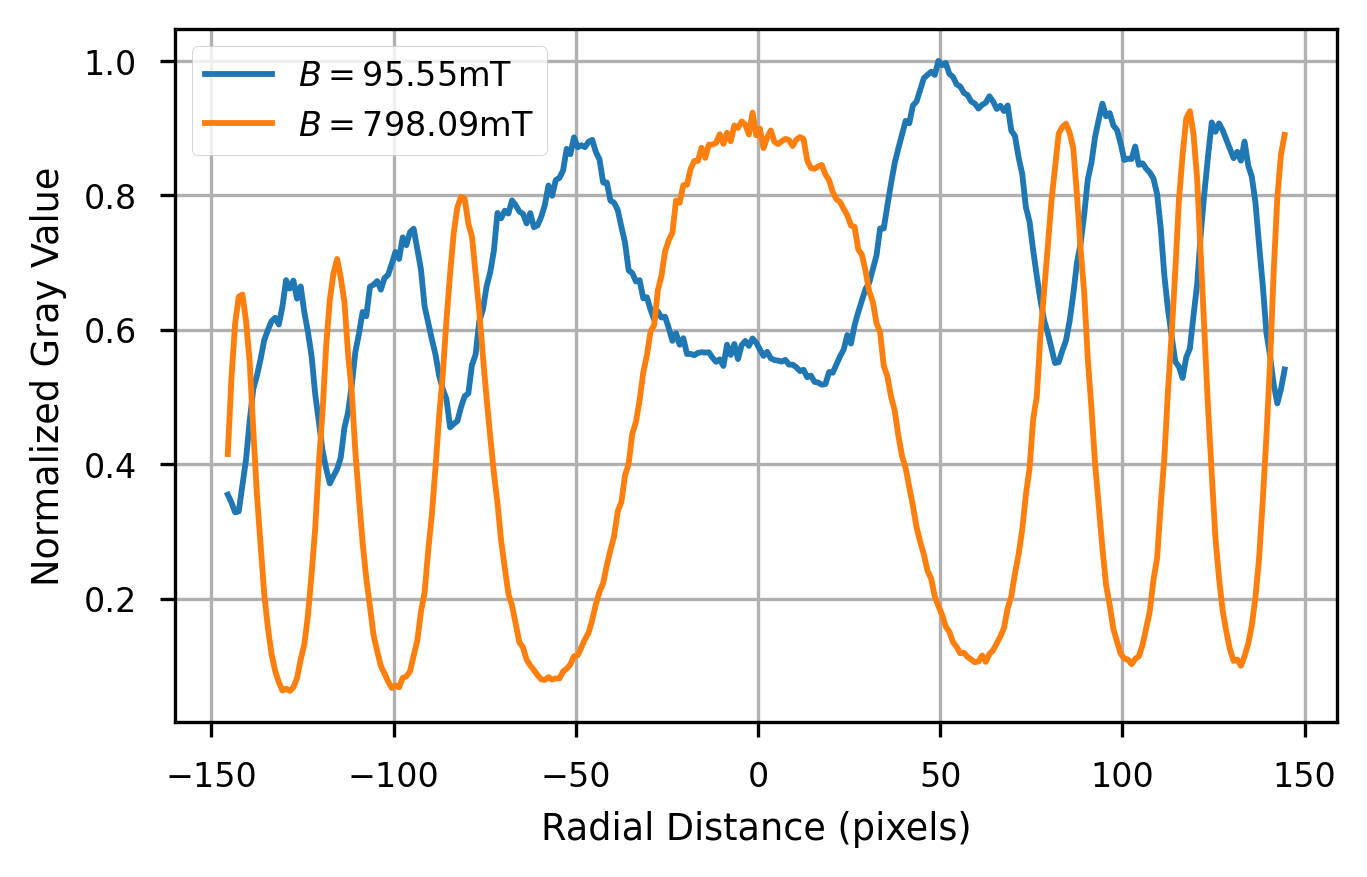
\includegraphics[width=0.75\linewidth]{figures//normal_zeeman_effect/zeemann_longitudinal_annormal_profile.png}
    \caption{Normalized intensity $I/I_\mathrm{max}$ as a function of radial distance from the ring center for the anomalous Zeeman effect in the longitudinal direction (without polarization filter) at $1\mathrm{A} \approx 95.55$mT and $10\text{A} \approx 798.09$mT.}
    \label{fig:zeemann_anomalous_longitudinal_profile}
\end{figure}

In the longitudinal direction, shown in figure~\ref{fig:zeemann_anomalous_longitudinal}, the situation is somewhat clearer. As shown in the normalized intensity profile, shown in figure~\ref{fig:zeemann_anomalous_longitudinal_profile}, the original single maximum at low field visibly broadens and begins to resolve into at least two distinct subpeaks at high field. This is consistent with the observation of the dominant $\sigma_\pm$ groups of lines, even if the full set of six longitudinal lines cannot be individually resolved. The energy separation between adjacent lines in the longitudinal anomalous case is $\frac{1}{2}\mu_B B$; at the maximum applied field of $B = 798$mT this amounts to approximately $\frac{1}{2}\times 9.274\times10^{-24}\times0.798 \approx 3.7\times10^{-24}$J. The experimental resolving limit is $\Delta E_\mathrm{min} = 2\mu_B B_m \approx 2\times9.274\times10^{-24}\times0.166 \approx 3.1\times10^{-24}$J. These two quantities are of comparable magnitude, so the anomalous lines at the highest available field are nearly at the edge of resolvability. The fact that only a partial splitting is observed—rather than a complete non-resolution—is therefore consistent with this marginal situation.

Figure~\ref{fig:zeemann_anomalous_transversal_polarization} shows the interference images recorded with a linear polarizer at angles $\theta = 0°$, $20°$, $45°$, and $90°$ at $B = 798.09$mT.

\begin{figure}[h]
    \centering
    
\includegraphics[width=0.75\linewidth]{figures//normal_zeeman_effect/zeemann_annormal_transversal_polarisation.png}
    \caption{Interference patterns of the anomalous Zeeman effect in the transversal direction with a linear polarizer at angles $\theta = [0°, 20°, 45°, 90°]$ at $B = 798.09$mT.}
    \label{fig:zeemann_anomalous_transversal_polarization}
\end{figure}

Rotation of the linear polarizer noticeably affects the width and intensity distribution of the observed rings, the rings are narrowest (most of the $\pi$ contribution is suppressed) at one angle and broadest (most of the $\sigma_\pm$ contribution is suppressed) at the orthogonal angle. Crucially, a residual ring is always visible regardless of the polarizer orientation, indicating that the transmitted light is not purely linearly polarized in a single direction. This is exactly what is expected in the transversal anomalous case, where $\pi$ lines that are linearly polarized parallel to $\vec{B}$) and $\sigma_\pm$ lines, that are linearly polarized perpendicular to $\vec{B}$ are simultaneously present and polarized orthogonally to each other. As neither set of lines can be resolved on its own, the polarizer alternately suppresses one group and transmits the other, according to Malus' law for a mixture of orthogonally polarized components.

\subsection{Resolving power}
\label{sec:resolving_power}

\subsubsection{Human criterion}

\begin{figure}[!ht]
    \begin{subfigure}{0.31\textwidth}
    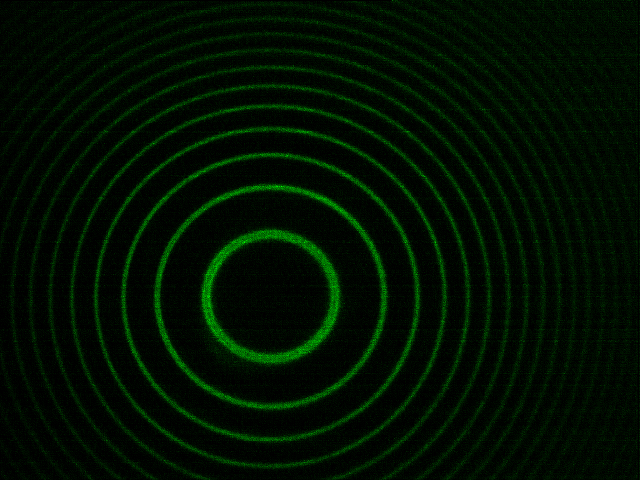
\includegraphics[width=1\linewidth]{figures//auflösevermögen/1_8A.png}
    \caption{$1.8$A ($\approx 158$mT)}
    \label{fig:auflösevermögen_1_8A}
    \end{subfigure}
    \begin{subfigure}{0.31\textwidth}
    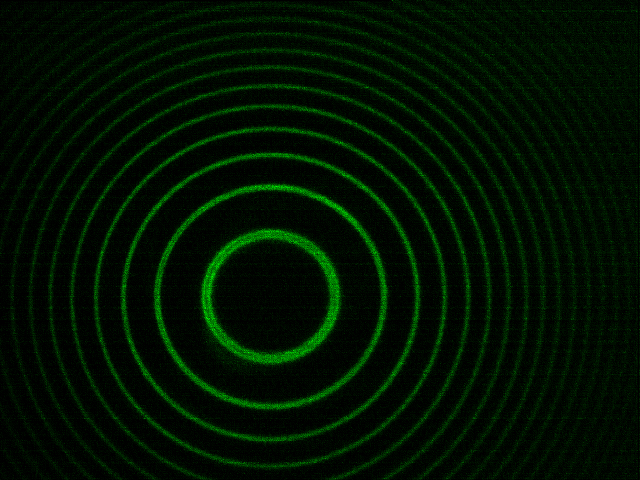
\includegraphics[width=1\linewidth]{figures//auflösevermögen/1_9A.png}
    \caption{$1.9$A ($\approx 166$mT)}
    \label{fig:auflösevermögen_1_9A}
    \end{subfigure}
    \begin{subfigure}{0.31\textwidth}
    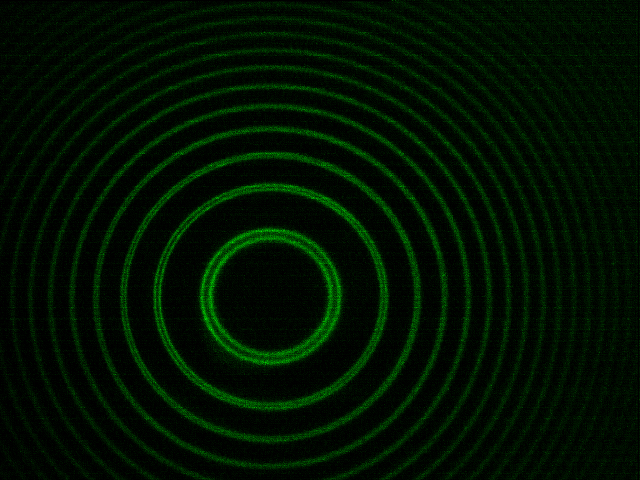
\includegraphics[width=1\linewidth]{figures//auflösevermögen/2_8A.png}
    \caption{$2.8$A ($\approx 236$mT)}
    \label{fig:auflösevermögen_2_8A}
    \end{subfigure}
\caption{Interference patterns of the normal Zeeman effect in the longitudinal configuration without a polarization filter at three different magnetic flux densities, used to determine the human criterion for the resolving power.}
\label{fig:human_crit}
\end{figure}

To determine the human criterion for the resolving power, the longitudinal configuration at $\lambda = 643.8$nm was used, since only two rings per order are visible because the $\pi$ ring is absent, making the onset of resolution straightforward to judge. The coil current was slowly increased while observing the CCD image in real time. The critical magnetic flux density $B_m$ was identified as the smallest field at which two separate rings per order could clearly be distinguished from a single merged ring. Based on the images in figure~\ref{fig:human_crit}, this threshold is at approximately $1.9$A, corresponding to $B_m \approx 166$mT according to equation~\eqref{current_to_flux_formula}

Because the $\pi$ ring is absent in the longitudinal configuration, the two visible rings are separated by twice the single-sublevel energy splitting: $\Delta E = 2\mu_B B_m$. Using equation~\eqref{eq:resolving_exp} with $\lambda = 643.8$nm and $\mu_B = 9.274 \cdot 10^{-24}$J/T, the human resolving power is

\begin{equation}
    \left(\frac{\lambda}{\Delta\lambda}\right)_\mathrm{human} = \frac{hc}{2\mu_B B_m\lambda} \approx 1.00 \cdot 10^5.
\end{equation}

\subsubsection{Technical criterion}

The technical criterion defines two peaks as resolvable when their separation equals the FWHM of a single peak. To determine the FWHM, the intensity profile of a well-separated single peak at large $B$, so that the two rings are far apart was fitted with a Gaussian function including a constant background offset to account for stray light:

\begin{equation}
    I(x) = I_\mathrm{max} \cdot \exp\!\left[-\frac{(x-x_0)^2}{2\sigma_2}\right] + I_0.
\end{equation}

\begin{figure}[h]
    \centering
    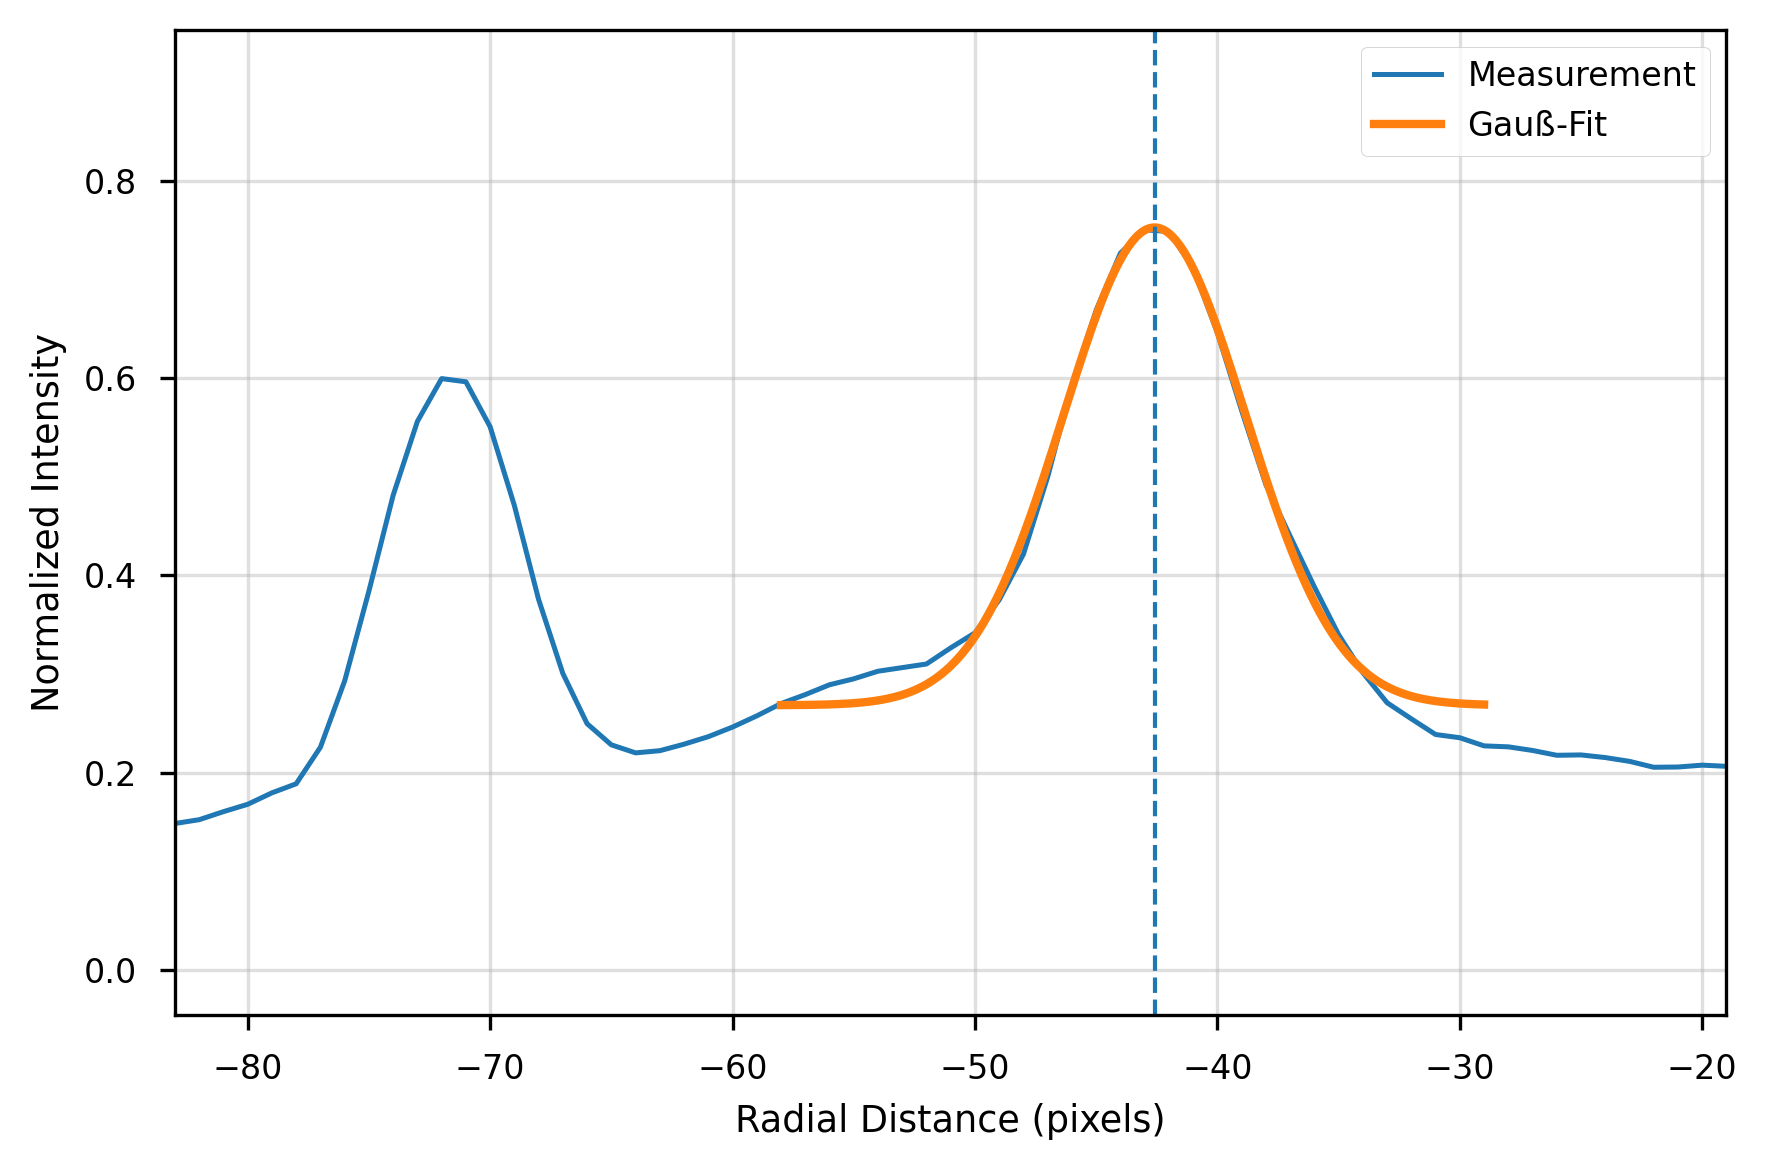
\includegraphics[width=0.75\linewidth]{figures//auflösevermögen/auflösungsvermögen_technisch.png}
    \caption{Intensity as a function of radial distance $r$ for the normal Zeeman effect in the longitudinal direction at $798.09$mT, with a Gaussian fit used to determine the FWHM of a single peak.}
    \label{fig:tech_crit}
\end{figure}

The Gaussian fit to the data shown in figure~\ref{fig:tech_crit} yields a standard deviation of

\begin{equation}
    \sigma = 3.762\mathrm{px}.
\end{equation}

The FWHM of the single peak is then

\begin{equation}
    \mathrm{FWHM} = 2\sqrt{2\ln 2}\cdot\sigma = 8.861\mathrm{px} \approx 9\mathrm{px}.
\end{equation}

To find the critical flux density $B_T$ for the technical criterion, the center-to-center separation between the two $\sigma_\pm$ rings in the radial intensity profile must be determined as a function of $B$. The two rings appear at radii $r_{1} = D_{1,1}/2$ and $r_{3} = D_{3,1}/2$, so their peak separation in the radial profile is $\Delta r = (D_{3,1} - D_{1,1})/2$. Using the ring diameters from Table~\ref{tab:bohr_magneton} because this is also the normal Zeeman effect in longitudinal configuration.

\begin{center}
\begin{tabular}{rr}
\toprule
$B$ [mT] & $\Delta r = (D_{3,1}-D_{1,1})/2$ [px] \\
\midrule
173.61 & 7.0 \\
251.67 & 8.5 \\
329.73 & 11.5 \\
\bottomrule
\end{tabular}
\end{center}

The two rings are just resolved by the technical criterion when $\Delta r = \mathrm{FWHM} = 9$px. Linear interpolation between the $B = 251.67$mT and $B = 329.73$mT entries yields

\begin{equation}
    B_T = 251.67 + \frac{9.0 - 8.5}{11.5 - 8.5}\times(329.73 - 251.67) \approx 265\mathrm{mT}.
\end{equation}

The technical resolving power is therefore

\begin{equation}
    \left(\frac{\lambda}{\Delta\lambda}\right)_\mathrm{tech} = \frac{hc}{2\mu_B B_T\lambda} = \frac{(6.626\cdot10^{-34})(3\cdot10^{8})}{2\cdot9.274\cdot10^{-24}\cdot0.265\cdot643.8\cdot10^{-9}} \approx 6.3\cdot 10^4.
\end{equation}

This value is significantly lower than the human threshold of $1.00 \cdot 10^5$. The difference comes down to perception and rigid definitions. The human eye can often tell two overlapping peaks apart even when they are closer than one FWHM (here, 7px vs. 9px at $B_m = 166$mT).

While the FWHM provides a conservative, instrument-based baseline, deciding when two peaks are truly "distinguishable" to a human viewer is ultimately subjective to the viewer.

\subsubsection{Theoretical resolving power}

The theoretical resolving power of the Fabry-Pérot interferometer is given by equation~\eqref{eq:resolving_theo}. With the interferometer parameters $d = 3$mm and $R = 0.9$, and evaluated at the two relevant wavelengths, one obtains:

For the normal Zeeman effect at $\lambda = 643.8$nm:
\begin{equation}
    \left(\frac{\lambda}{\Delta\lambda}\right)_\mathrm{theo} = \frac{2\pi \cdot 0.003\mathrm{m} \cdot \sqrt{0.9}}{643.8 \cdot 10^{-9}\mathrm{m} \cdot (1 - 0.9)} \approx 2.78 \cdot 10^5.
\end{equation}

The experimentally determined resolving power is approximately a factor of 2.8 smaller than the theoretical value at $\lambda = 643.8$nm. Several physical effects contribute to this discrepancy. First, the theoretical formula assumes perfectly flat mirrors with an ideal reflectivity $R$ that is uniform over the entire surface. In practice, surface roughness and slight non-parallelism of the mirror plates introduce additional phase errors that broaden the transmission peaks and reduce the effective finesse. Second, the cadmium lamp does not emit perfectly monochromatic radiation. Doppler broadening from the thermal motion of the atoms in the hot gas contribute a natural line width, which sets an lower bound on the resolvable wavelength difference independent of the interferometer. Finally, the limited pixel size and read noise of the CCD sensor has uncertainties in reading the ring positions. All these effects together explain why the experimental resolving power is reduced by roughly a factor of 3 relative to the ideal theoretical limit.

\subsection{Bohr magneton}

The Bohr magneton $\mu_B$ is determined from the longitudinal configuration of the normal Zeeman effect, where the energy splitting between adjacent sublevels is $\Delta E = \mu_B B$. As derived in Section~\ref{sec:fabrypérot}, the energy difference between the inner ($\sigma_-$) and outer ($\sigma_+$) rings observed in the longitudinal case is $\Delta E_\mathrm{obs} = 2\mu_B B$. Accordingly, the relevant formula for extracting $\mu_B$ from the measured ring diameters is

\begin{equation}
    \Delta E = \frac{hc}{4d}\left|\frac{D_{1,m}^2}{D_{1,m+1}^2 - D_{1,m}^2} - \frac{D_{3,m}^2}{D_{3,m+1}^2 - D_{3,m}^2}\right| = \mu_B B,
    \label{bohr_magneton_formula}
\end{equation}

where $D_{1,m}$ and $D_{3,m}$ are the diameters of the outer and inner $\sigma$ rings in interference order $m$, and $D_{1,m+1}$, $D_{3,m+1}$ are their counterparts in the adjacent order $m+1$ like in figure~\ref{fig:ring_explain} shown. The absolute value is taken because the sign of the bracket depends only on the labeling convention of the ring orders and carries no physical meaning. The energy splitting is by definition positive.

\begin{figure}
    \centering
    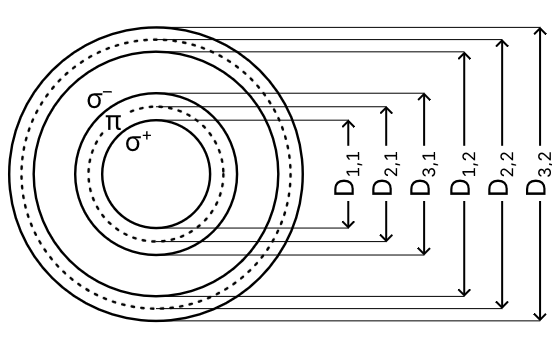
\includegraphics[width=0.75\linewidth]{figures/explaining_of_diameter.png}
    \caption{Illustration of the different interference ring diameters for two interference orders}
    \label{fig:ring_explain}
\end{figure}

The measurement uncertainty on each ring diameter is estimated as $\pm 1$pixel, limited by the CCD pixel size and the precision of the ImageJ measurement tool, and a relative uncertainty of 1\% is assumed for the magnetic flux density $B$ because of the fit uncertainty.

The ring diameters were extracted from the interference images using ImageJ, and the results are listed in Table~\ref{tab:bohr_magneton}.

\begin{table}[!ht]
    \centering
    \begin{tabular}{rrrrrll}
        B [mT] & $D_{1,1} [px]$ & $D_{3,1} [px]$ & $D_{1,2} [px]$ & $D_{3,2} [px]$ & $\Delta E$ [J] & Error $\Delta E$ [J] \\ \hline \hline
        173.61 & 122 & 136 & 224 & 229 & $2.04\cdot 10^{-24}$ & $3.02\cdot 10^{-25}$ \\ \hline
        251.67 & 121 & 138 & 222 & 231 & $2.19\cdot 10^{-24}$ & $3.06\cdot 10^{-25}$ \\ \hline
        329.73 & 117 & 140 & 220 & 233 & $2.82\cdot 10^{-24}$ & $3.01\cdot 10^{-25}$ \\ \hline
        407.79 & 114 & 143 & 218 & 235 & $3.50\cdot 10^{-24}$ & $3.05\cdot 10^{-25}$ \\ \hline
        485.85 & 111 & 146 & 216 & 238 & $4.05\cdot 10^{-24}$ & $3.05\cdot 10^{-25}$ \\ \hline
        563.91 & 107 & 150 & 214 & 239 & $5.24\cdot 10^{-24}$ & $3.19\cdot 10^{-25}$ \\ \hline
        641.97 & 105 & 152 & 213 & 241 & $5.62\cdot 10^{-24}$ & $3.19\cdot 10^{-25}$ \\ \hline
        720.03 & 102 & 154 & 211 & 241 & $6.38\cdot 10^{-24}$ & $3.31\cdot 10^{-25}$ \\ \hline
        798.09 & 98 & 156 & 210 & 243 & $6.99\cdot 10^{-24}$ & $3.29\cdot 10^{-25}$ \\ \hline
    \end{tabular}
    \caption{Measured ring diameters in pixels for the normal Zeeman effect in the longitudinal configuration, together with the computed energy splitting $\Delta E$ using equation~\eqref{bohr_magneton_formula} with $d = 3$mm}
    \label{tab:bohr_magneton}
\end{table}

\begin{figure}[h]
    \centering
    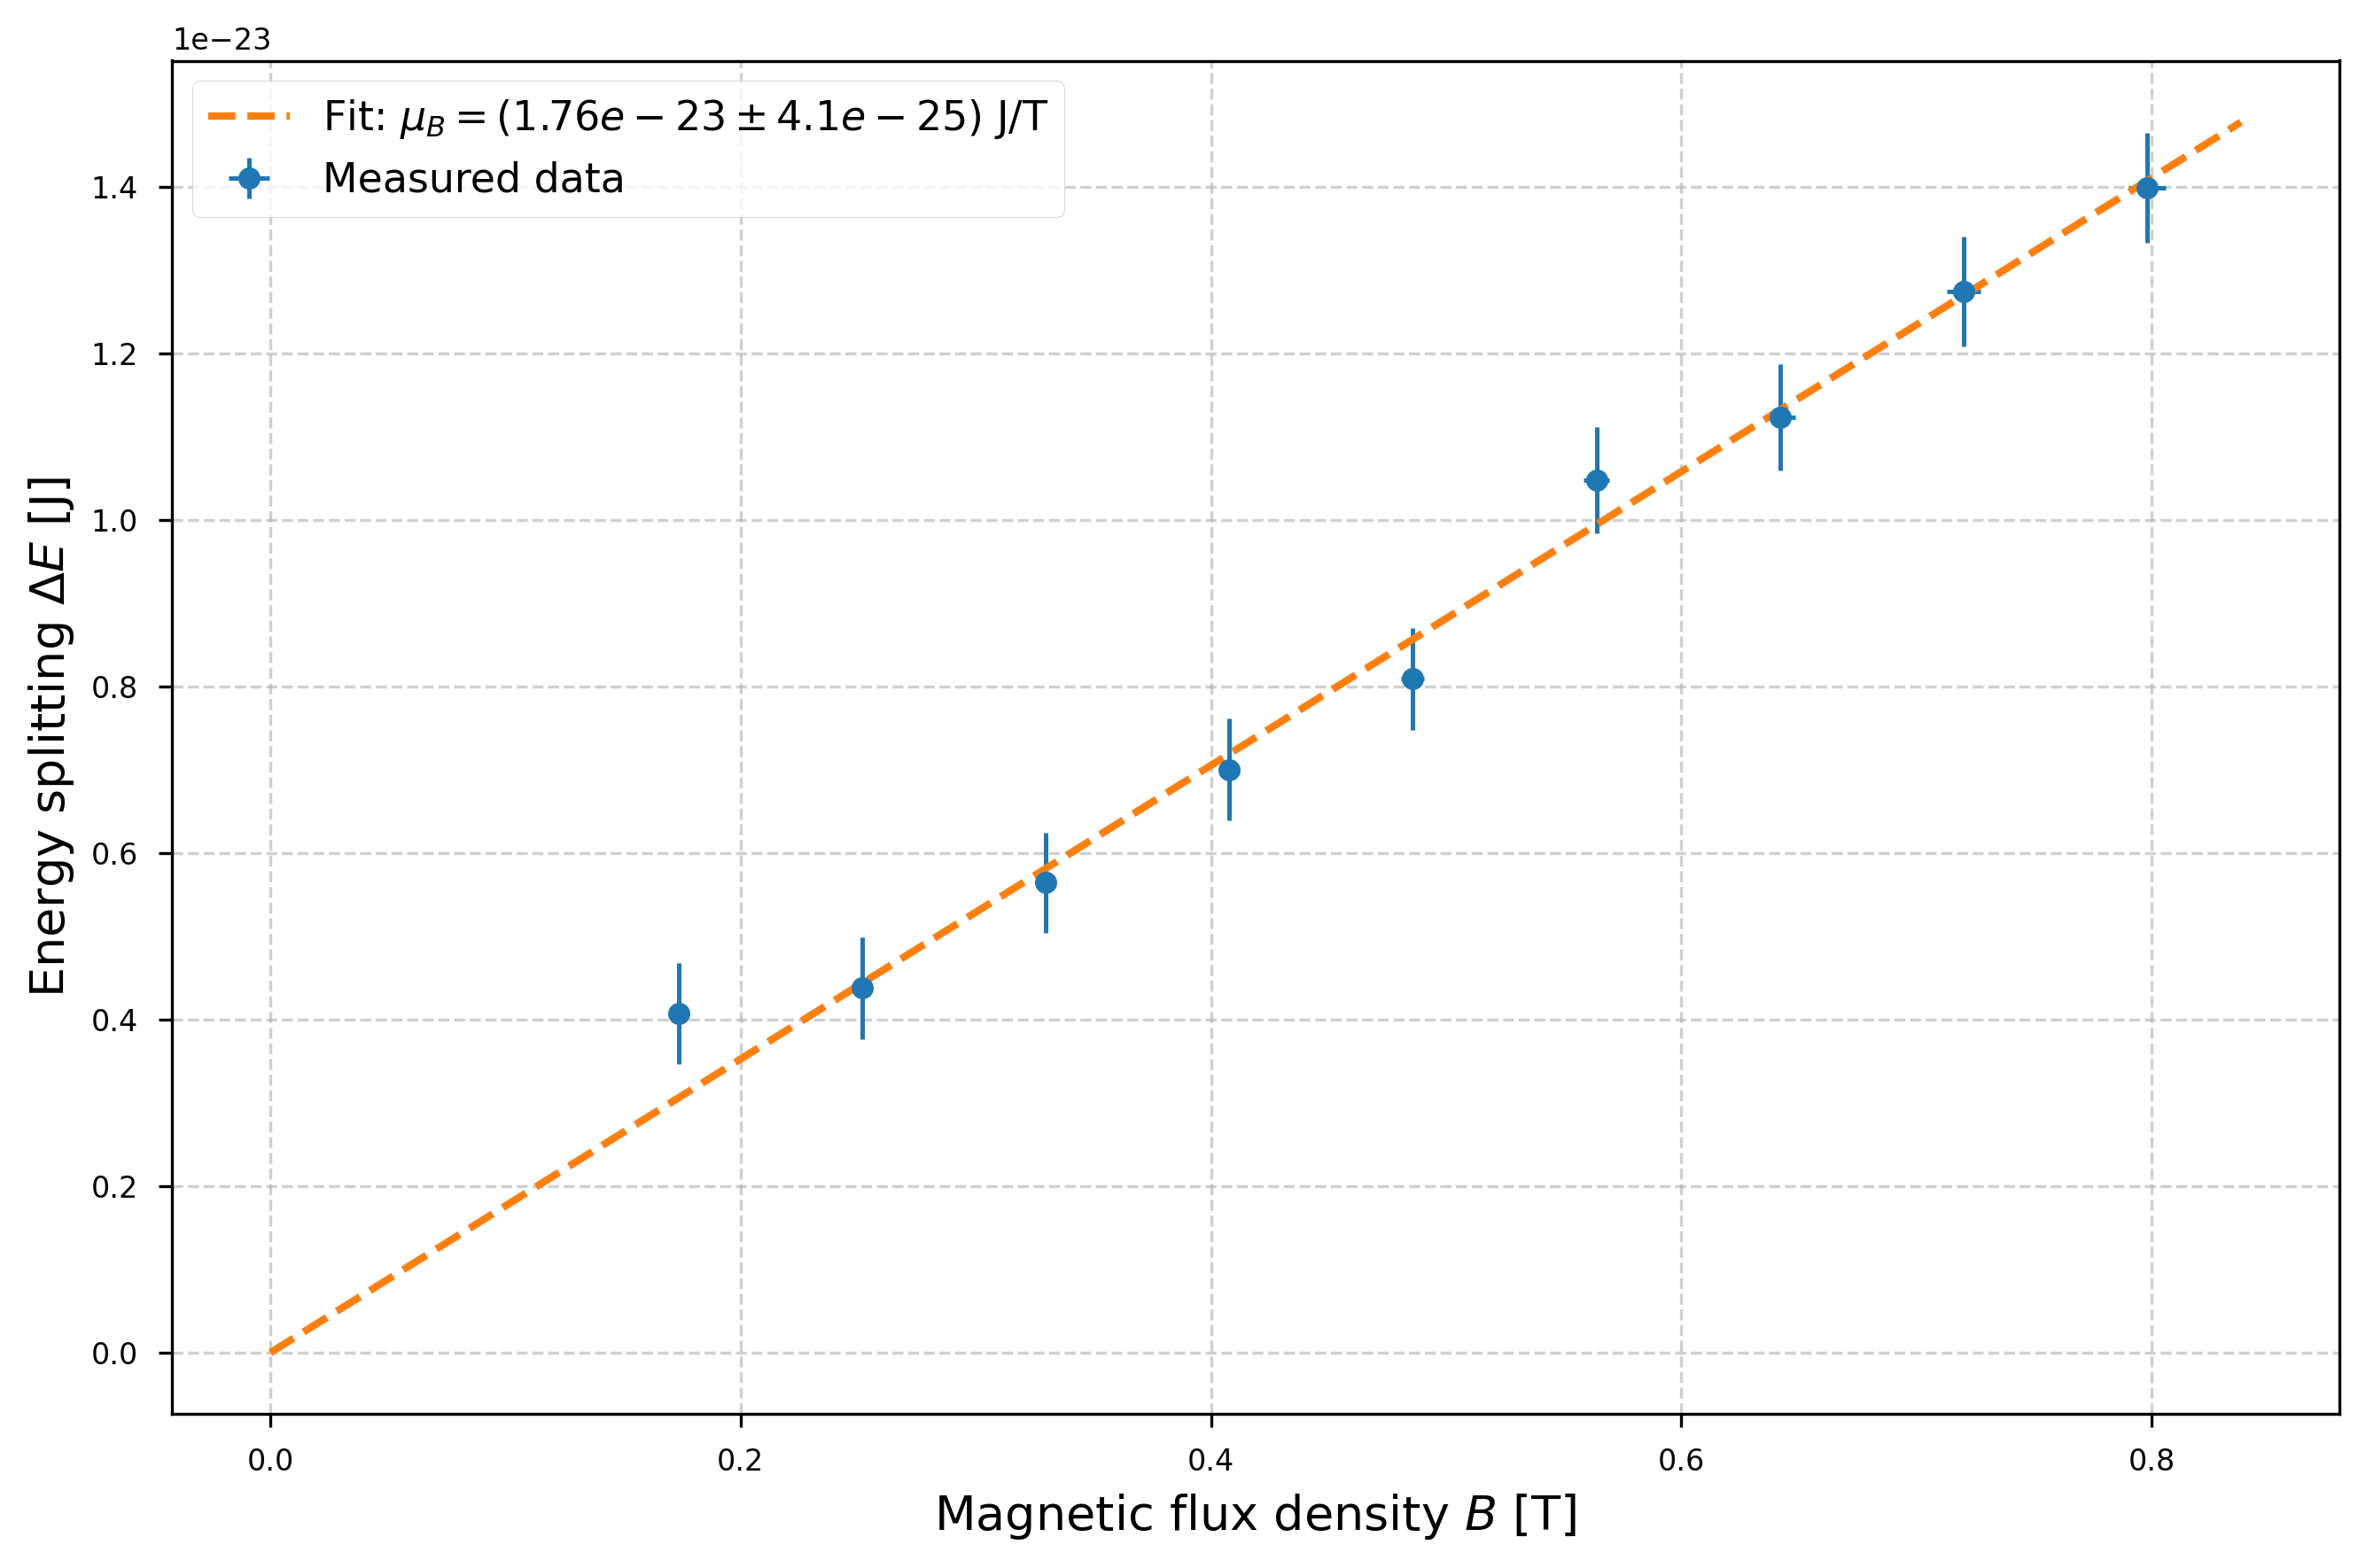
\includegraphics[width=0.75\linewidth]{figures//magneton/magneton_plot.png}
    \caption{Zeeman energy splitting $\Delta E$ as a function of the magnetic flux density $B$, with a linear fit to determine the Bohr magneton $\mu_B$.}
    \label{fig:bohr_magneton}
\end{figure}

The energy splitting $\Delta E$ is plotted as a function of $B$ in figure~\ref{fig:bohr_magneton}. According to equation~\eqref{bohr_magneton_formula}, $\Delta E$ and $B$ are related by $\Delta E = \mu_B B$, so the slope of a linear fit through the origin directly yields $\mu_B$. The fit gives

\begin{equation}
   \mu_B^\mathrm{exp} = (8.82 \pm 0.20) \cdot 10^{-24}J/T.
\end{equation}

The accepted literature value is
\begin{equation}
    \mu_{B,\mathrm{ref}} = \frac{e\hbar}{2m_e} = 9.274 \cdot 10^{-24}J/T.
\end{equation}
The experimental value is in good agreement with the literature value, with a relative deviation of 4.90\%.

Sources of systematic error include the uncertainty in the mirror spacing $d$, the calibration uncertainty of the magnetic field, and the limited precision with which ring diameters can be determined from pixelated CCD images. 
The pixel-size uncertainty of $\pm 1$px enters equation~\eqref{bohr_magneton_formula} nonlinearly through the quadratic terms $D^2$, making it particularly important for rings of small diameter.

Despite these contributions, the corrected result is in good agreement with the literature value.

\section{Summary and Outlook}

In this experiment, the Zeeman effect was investigated comprehensively using a cadmium spectral lamp, an electromagnet, and a Fabry-Pérot interferometer. The magnetic field between the pole pieces was calibrated using a Hall effect sensor, yielding a linear calibration function $B(I) = 78.06\mathrm{mT/A} \cdot I + 17.49$mT, which is valid over the full range of currents used (0A to 10A) with a maximum deviation of less than 10\%. The spatial profile of the field showed a maximum at the center of the gap with a symmetric decrease towards the pole-piece edges due to fringing; the variation across the active volume of the cadmium lamp was well below 10\%, so the field could be treated as sufficiently homogeneous.

For the normal Zeeman effect at $\lambda = 643.8$nm ($3^1D_2 \leftrightarrow 2^1P_1$ transition, $S=0$), the expected triplet splitting was clearly observed in the transversal configuration, and the doublet splitting (without the central $\pi$ ring) in the longitudinal configuration. Polarization analysis using a linear polarizer and a quarter-wave plate confirmed that the $\pi$ component is linearly polarized parallel to $\vec{B}$ and the $\sigma_\pm$ components are linearly polarized perpendicular to $\vec{B}$ in the transversal direction, and circularly polarized (with opposite helicity) in the longitudinal direction—in complete agreement with theory.

For the anomalous Zeeman effect at $\lambda = 508.6$nm ($2^3S_1 \leftrightarrow 2^3P_2$ transition, $S=1$), the theoretically expected nine lines in the transversal direction and six lines in the longitudinal direction could not be fully resolved individually, because the sub-level energy spacing $\frac{1}{2}\mu_B B$ is smaller than the experimental resolving power. However, a clear broadening and partial splitting of the rings with increasing field was observed, consistent with the anomalous pattern.

The resolving power of the optical setup was determined experimentally using two independent criteria. The human criterion, based on visual inspection of the interference images, yielded $\lambda/\Delta\lambda \approx 1.00\cdot 10^5$ at a critical flux density of $B_m \approx 166$mT. The technical criterion, defined as the field at which the ring separation equals the FWHM of a single peak (9px), gives $B_T \approx 265$mT and a corresponding resolving power of $\lambda/\Delta\lambda \approx 6.3\cdot 10^4$. The two criteria yield different values, as expected. The human eye can perceive two rings as separate even when their radial separation is somewhat less than one FWHM, resulting in a higher apparent resolving power. The theoretical maximum resolving power of the Fabry-Pérot interferometer at $\lambda = 643.8$nm is $2.78\cdot 10^5$, approximately a factor of 4 larger than the technical criterion result. The discrepancy is attributed to imperfect mirror parallelism, surface roughness, acoustic vibrations, the natural linewidth of the cadmium emission, and the finite CCD pixel size.

The Bohr magneton was extracted from a linear fit to the Zeeman energy splitting as a function of magnetic flux density, using the correct formula for the longitudinal configuration with the factor $4d$ in the denominator. The fit yields $\mu_B^\mathrm{exp} = (8.82 \pm 0.20)\cdot10^{-24}$J/T, in good agreement with the literature value $\mu_{B,\mathrm{ref}} = 9.274\cdot10^{-24}$J/T to within 4.90\%. This deviation is within the $1\sigma$ uncertainty of the linear fit, confirming the consistency of the result.

The observation that the overall brightness of the cadmium lamp increased with increasing coil current is likely due to the Lorentz force acting on the ions in the plasma. The stronger magnetic field compresses the ions to a smaller volume, which increases the collision rate with neutral atoms and thus the excitation rate and intensity of the emitted light.

One possible improvement for the future would be to increase the mirror spacing $d$ or the mirror reflectivity $R$ to increase the resolving power of the interferometer. Another would be to determine the ring diameters with sub-pixel precision by fitting Gaussian profiles to the radial intensity peaks, instead of reading peak positions by eye in ImageJ, and this would reduce the systematic measurement error in the determination of the Bohr magneton.

\newpage
\listoffigures
\listoftables

\nocite{*}
\printbibliography

\end{document}